\documentclass[10pt]{beamer}
\usepackage[utf8]{inputenc}
\usetheme{Madrid}
\usecolortheme{crane}
\usepackage{esvect}
\usepackage{amsmath}
\usepackage{mathrsfs}
\usepackage{amssymb}
\usepackage{dsfont}
\usepackage{physics}
\usepackage{amsmath, amssymb, amsthm, float, graphicx, amsfonts}
\usepackage{relsize}
\newcommand\hmmax{0}
\newcommand\bmmax{0} 
%\usepackage[unicode]{hyperref}
\usepackage{amsmath}
\usepackage[bottom]{footmisc}
%\usepackage{showkeys}
\usepackage{graphicx}
\usepackage{mwe}
\usepackage[section]{placeins}
\usepackage{framed}
\usepackage{csquotes}
\usepackage{tikz}
\usetikzlibrary{decorations.markings}
\usetikzlibrary{decorations.pathmorphing}
\definecolor{shadecolor}{rgb}{0.90,0.90,0.90}
%\usepackage{natbib}
\usepackage{cite}
%\usepackage[linkbordercolor=blue]{hyperref}
\usepackage{hyperref}
\usepackage{bbold}
%\usepackage{wick}
\usepackage{subcaption}
\usepackage{pifont}
%\usepackage{dingbat}
%\usepackage{mathtools}
\usepackage{setspace}
\usepackage{amsmath, amssymb, amsthm, float, graphicx,amsfonts}
\usepackage{MnSymbol}
\numberwithin{equation}{section}
%t\usepackage{wasysym}
%\setlength{\unitlength}{1mm}
%\DeclareMathOperator{\arccsc}{arccsc}
\usepackage{amsthm}
\usepackage{array, boldline, makecell, booktabs}
\newcommand\btrule[1]{\specialrule{#1}{0pt}{0pt}}
\setlength{\arrayrulewidth}{0.5mm}
\setlength{\tabcolsep}{10pt}
\renewcommand{\arraystretch}{1.4}
\setbeamertemplate{caption}[numbered]

\parskip=9pt
\setbeamercolor{emph}{fg=red}
\renewcommand<>{\emph}[1]{%
  {\usebeamercolor[fg]{emph}\only#2{\itshape}#1}%
}



\def\beq{\begin{eqnarray}}\def\eeq{\end{eqnarray}}
\def\be{\begin{equation}}\def\ee{\end{equation}}
\def\minusp{{\mp}}
\def\a{\alpha}
\def\b{\beta}
\def\c{\chi}
\def\d{\delta}
\def\e{\epsilon}
\def\ve{\varepsilon}
\def\f{\phi}
\def\g{\gamma}
\def\h{\eta}
\def\i{\iota}
\def\k{\kappa}
\def\l{\lambda}
\def\L{\Lambda}
\def\m{\mu}
\def\n{\nu}
\def\p{\pi}
\def\ps{\psi}
\def\r{\rho}
\def\s{\sigma}
\def\t{\tau}
\def\th{\theta}
\def\w{\omega}
\def\x{\xi}
\def\z{\zeta}
\def\D{\Delta}
\def\F{\Phi}
\def\P{\Pi}
\def\G{\Gamma}
\def\W{\Omega}
\def\Th{\Theta}
\def\pd{\partial}
\def\tq{\tilde{q}}
\def\tf{\tilde{f}}
\def\bz{\bar{z}}
\def\la{\langle}
\def\ra{\rangle}
\def\vf{\varphi}
\def\fin{f_{\infty}}
\def\ma{{\mathcal{A}}}
\def\mb{{\mathcal{B}}}
\def\mc{{\mathcal{C}}}
\def\md{{\mathcal{D}}}
\def\me{{\mathcal{E}}}
\def\mf{{\mathcal{F}}}
\def\mg{{\mathcal{G}}}
\def\mh{{\mathcal{H}}}
\def\mi{{\mathcal{I}}}
\def\mj{{\mathcal{J}}}
\def\mk{{\mathcal{K}}}
\def\ml{{\mathcal{L}}}
\def\mm{{\mathcal{M}}}
\def\mn{{\mathcal{N}}}
\def\mo{{\mathcal{O}}}
\def\mp{{\mathcal{P}}}
\def\mq{{\mathcal{Q}}}
\def\mr{{\mathcal{R}}}
\def\ms{{\mathcal{S}}}
\def\mt{{\mathcal{T}}}
\def\mw{{\mathcal{W}}}
\def\mz{{\mathcal{Z}}}
\def\fA{\mathfrak{A}}
\def\fB{\mathfrak{B}}
\def\fN{{\mathfrak{N}}}
\def\fQ{{\mathfrak{Q}}}
\def\ff{{\mathfrak{f}}}
\def\lan{\langle}
\def\ran{\rangle}
\def\pb{\textbf{P}}
\def\nb{\textbf{n}}
\def\xb{\textbf{x}}
\def\yb{\textbf{y}}
\def\Db{\textbf{D}}
\def\Kb{\textbf{K}}
\def\Pb{\textbf{P}}
\def\Mb{\textbf{M}}
\def\Lb{\textbf{L}}
\def\bh{\bar{h}}
\def\sb{\bar{s}}
\def\ib{{\mathbb{I}}}
\def\rb{\mathbb{R}}
\def\tell{\tilde{\ell}}
\def\tr{{\rm tr~}}
\def\nn{\nonumber}
\def\Mack{\widehat{\mathcal{P}}}
\def\MackQ{\widehat{\mq}}
\def\dphi{\D_\f}
\def\tmn{\tau_{\text{min}}}
\def\lsumf{\sum_{\substack{\ell\\ \ell~\text{even}}}}
\def\lsump{\sum_{\substack{\ell=L+2\\ \ell~\text{even}}}^\infty}
\def\lsumt{\sum_{\substack{\ell\\ \ell~\text{even}}}^L}
\def\kket#1{\mathinner{|{#1}\rrangle}}
\def\bbra#1{\mathinner{\llangle{#1}|}}
\def\bbrakket#1{\mathinner{\llangle{#1}\rrangle}}
\def\bbraket#1{\mathinner{\llangle{#1}\rangle}}
\def\brakket#1{\mathinner{\langle{#1}\rrangle}}
\def\lsumf{\sum_{\substack{\ell\\ \ell~\text{even}}}}
\def\lsump{\sum_{\substack{\ell=L+2\\ \ell~\text{even}}}^\infty}
\def\lsumt{\sum_{\substack{\ell\\ \ell~\text{even}}}^L}
\def\kket#1{\mathinner{|{#1}\rrangle}}
\def\bbra#1{\mathinner{\llangle{#1}|}}
\def\bbrakket#1{\mathinner{\llangle{#1}\rrangle}}
\def\bbraket#1{\mathinner{\llangle{#1}\rangle}}
\def\brakket#1{\mathinner{\langle{#1}\rrangle}}
\newcommand{\floor}[1]{\lfloor #1 \rfloor}
\newcommand{\ceil}[1]{\lceil #1 \rceil}
\newcommand{\bs}[1]{\boldsymbol{#1}}
\newcommand{\eq}[1]{eq.\eqref{#1}}
\newcommand{\Eq}[1]{Eq.\eqref{#1}}
\def\tenp{\otimes}
\def\tens{\oplus}
\usepackage{bm}
\usepackage{bm}

\title{S-matrix Bootstrap and Bounds on Wilson Coeff.}
\author{\textbf{Vinay Vikramaditya}}
\institute[UG IISc]{{\textbf{ \larger\\
  under \\
  Prof. Aninda Sinha\\
  CHEP, IISc Bangalore
\date{}
}}}



\begin{document}

\maketitle

\begin{frame}{Contents}
\tableofcontents
\end{frame}


\section{Introduction}
\begin{frame}{Introduction}
    \begin{itemize}
        \item Bootstrap is the use of minimal set of principles to constrain physical observables.
        \vspace{6pt}
        \item Its a non-pertubative method using properties like unitarity, crossing symmetry in general and poles due to prescence of bound states, resonances etc. dependending on which theory is in consideration.
        \vspace{6pt}
         \item Bootstrap was popular in the 1960s but fell out of favour after strong forces was succesfully described by non-abelian gauge theories. It was later revived for use in CFTs as conformal bootstrap in the 1970s and very recently (2016) the S-matrix bootstrap for QFTs.
	\vspace{6pt}
         \item Here we shall be looking at numerical bootstrap methods elucidated in [1],[2] using Semi-Definite Program Solver (SDPB) [3].
        \end{itemize}
        \vspace{60pt}
        
 
\end{frame}



\section{Pion Bootstrap}


\begin{frame}{Pion Bootstrap}
\framesubtitle{Invariant Tensors in $O(3)$}
    \begin{itemize}
        \item The $2\rightarrow 2$ scattering amplitude will have four indices and can be written in terms of 3 invariant tensors of $O(3)$ vector representation. \[ \mathcal{T}_{a b}^{c d}=A(s|t, u) \delta_{a b} \delta^{c d}+A(t|s, u) \delta_{a}^{c} \delta_{b}^{d} +A(u|s, t) \delta_{a}^{d} \delta_{b}^{c} \]
 \begin{figure}
    \centering
    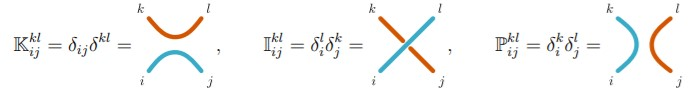
\includegraphics[width=0.8\textwidth]{1.jpg}
\end{figure}
	\item \( \mathds{P}_{\text {sing }}=\mathds{P}_{0}=\frac{1}{3} \delta_{a b} \delta^{c d}, \mathds{P}_{\text {anti }}=\mathds{P}_{1}=\frac{1}{2}\left(\delta_{a}^{c} \delta_{b}^{d}-\delta_{a}^{d} \delta_{b}^{c}\right), \mathds{P}_{\text {sym }}=\mathds{P}_{2}=\frac{1}{2}\left(\delta_{a}^{c} \delta_{b}^{d}+\delta_{a}^{d} \delta_{b}^{c}-\frac{2}{3} \delta_{a b} \delta^{c d}\right) \) following \( \mathds{P}_{I} \mathds{P}_{J}=\delta_{I J}\mathds{P}_{I} \)
	\item The scattering amplitude in terms of projection operators 
        \begin{equation*}
    \begin{split}
      \mathcal{T}=&(3 A(s|t, u)+A(t|s, u)+A(u|s, t)) \mathds{P}_{0} \\
&+(A(t|s, u)-A(u|s, t)) \mathds{P}_{1}+(A(t|s, u)+A(u|s, t)) \mathds{P}_{2} \\
=& \mathcal{T}^{(0)} \mathds{P}_{0}+ \mathcal{T}^{(1)} \mathds{P}_{1}+ \mathcal{T}^{(2)} \mathds{P}_{2} 
     \end{split}
    \end{equation*}
    \end{itemize}
\end{frame}




\begin{frame}{Pion Bootstrap}
\framesubtitle{Partial Wave Unitarity}
    \begin{itemize}
	\item \( S_{\ell}^{(I)}(s)=1+\left.i \frac{\sqrt{s-4}}{\sqrt{s}} \int_{-1}^{1} d x \frac{P_{\ell}(x)}{32 \pi} \mathcal{T}^{(I)}(s, t)\right|_{t \rightarrow \frac{1}{2}(s-4)(x-1)}=1+2 i \frac{\sqrt{s-4}}{\sqrt{s}} \mathcal{T}_{l}^{(I)} \) 
	\item Optical theorem  \[ \operatorname{Im} \mathcal{T}(\pi \pi \rightarrow \pi \pi)  \geq 2 E_{C M}\left|\vec{p}_{i}\right| \frac{1}{64 \pi E_{CM}^{2}} \int d(\cos \theta)|\mathcal{T}(\pi \pi \rightarrow \pi \pi)|^{2} \]
       \item Since \( \mathds{P}_{I} \mathds{P}_{J}=\delta_{I J}\mathds{P}_{I} \), \[  \operatorname{Im} \mathcal{T}^{(I)}(\pi \pi \rightarrow \pi \pi)  \geq 2 E_{C M}\left|\vec{p}_{i}\right| \frac{1}{64 \pi E_{CM}^{2}} \int d(\cos \theta)|\mathcal{T}^{(I)}(\pi \pi \rightarrow \pi \pi)|^{2} \]
	\item Expanding using \(\mathcal{T}^{(I)}=32 \pi \sum_{\ell} \mathcal{T}^{(I)}_{\ell}(2 \ell+1) P_{\ell}(\cos (\theta))\)  gives \( \operatorname{Im}\left(\mathcal{T}^{(I)}_{l}\right) \geq \frac{\sqrt{s-4}}{\sqrt{s}} \left|\mathcal{T}^{(I)}_{l}\right|^{2}  \) which using \( \mathcal{T}_{l}^{(I)}=\frac{S_{l}^{(I)}(s)-1}{2 i} \frac{\sqrt{s}}{\sqrt{s-4}} \) implies the partial wave unitarity condition \[ \left|S^{(I)}_{l}(s)\right|^{2} \leq 1 \]
    \end{itemize}
\end{frame}

\begin{frame}{Pion Bootstrap [2] \footnote[frame]{M. F. Paulos, J. Penedones, J. Toledo, B. C. van Rees and P. Vieira, “The S-matrix Bootstrap III: Higher Dimensional Amplitudes,” arXiv:1708.06765}}
	
    We use a transformation to map the cut $s$-plane to a unit disk and similar transformation for $t$ and $u$:
   \[ s \mapsto \rho_{s}=\frac{\sqrt{4 m^{2}-s_{0}}-\sqrt{4 m^{2}-s}}{\sqrt{4 m^{2}-s_{0}}+\sqrt{4 m^{2}-s}}, \quad s=\frac{s_{0}\left(1-\rho_{s}\right)^{2}+16 m^{2} \rho_{s}}{\left(1+\rho_{s}\right)^{2}}\]
   \begin{figure}
    \centering
    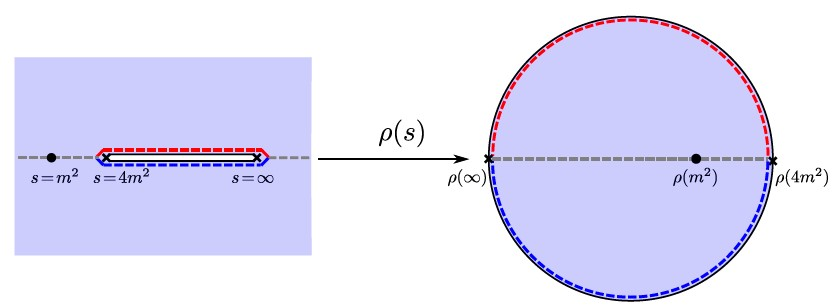
\includegraphics[width=0.6\textwidth]{2.jpg}
\end{figure}
This helps since the unit disk isk is a finite region, and the branch cut maps to boundary of this unit disk. 
\end{frame}


\begin{frame}{Pion Bootstrap [1]\footnote[frame]{A. L. Guerrieri, J. Penedones, P. Vieira, "Bootstrapping QCD: the Lake, the Peninsula and the Kink" arxiv:1810.12849}}
\framesubtitle{Ansatz}
	\begin{itemize}
	\item Crossing symmetry for a process $a\left(p_{a}\right)+b\left(p_{b}\right) \rightarrow$ $c\left(p_{c}\right)+d\left(p_{d}\right)$ with amplitude \( \mathcal{T}_{a b}^{c d}=A(s|t, u) \delta_{a b} \delta^{c d}+A(t|s, u) \delta_{a}^{c} \delta_{b}^{d} +A(u|s, t) \delta_{a}^{d} \delta_{b}^{c} \) can be found by interchanging $c\leftrightarrow d$ which interchanges $t\leftrightarrow u$ and comparing coeff. of the invariant tensors to get $A(s|t, u)=A(s|u,t)$ and by crossing in other ways, we can show that $A(x|y,z)=A(x|z,y)$ for any Mandelstram variables.
\vspace{6pts}
	\item So a crossing symmetric analytic (in the disk) ansatz for $A(s|t, u)$ in terms of the new variables in abscence of poles/bound states is \[A(s | t, u)=\sum_{n \leq m}^{\infty} a_{n m}\left(\rho_{t}^{n} \rho_{u}^{m}+\rho_{t}^{m} \rho_{u}^{n}\right)+\sum_{n, m}^{\infty} b_{n m}\left(\rho_{t}^{n}+\rho_{u}^{n}\right) \rho_{s}^{m}\] with $\rho_{z} = \frac{\sqrt{\frac{8}{3}}-\sqrt{4-z}}{\sqrt{\frac{8}{3}}+\sqrt{4-z}}$.

	\end{itemize}    
\end{frame}


\begin{frame}{SDPB [3]\footnote[frame]{D. Simmons-Duffin, "A Semi-definite Program Solver for the Conformal Bootstrap" arXiv:1502.02033}}
\framesubtitle{Unitarity}
	\begin{itemize}
	\item SDPB solves the following problem
	\begin{equation*}
    \begin{split}
      &\text { maximize } a \cdot z \text { over } z \in \mathds{R}^{N+1},\\
&\text { such that } \sum_{n=0}^{N} z_{n} W_{j}^{n}(x) \succeq 0 \quad \text { for all } x \geq 0 \text { and } 1 \leq j \leq J\\
&\text{ with normalization }n\cdot z=1
     \end{split}
    \end{equation*}

	\item To use this to impose unitarity, we first begin by writing $\mathcal{T}(s, t, 4-s-t)=\vec{\eta} \cdot \vec{\mathcal{T}}(s, t)$ where $\vec{\eta}$ is a vector containing all parameters in the ansatz (like all $a_{n m}, b_{n m}$ in case of pion bootstrap).
        \item Suppresing isospin index, unitarity $|S_{l}(s)|^{2}\leq 1$ with definitions $\vec{R}=\operatorname{Re}\left[\vec{\mathcal{T}_{\ell}(s)}\right]$ and $\vec{I}=\operatorname{Im}\left[\vec{\mathcal{T}_{\ell}(s)}\right]$, is equivalent to semidefiniteness of \[ M:=\left(\begin{array}{cc}
1+\vec{\eta} \cdot \vec{R} & 1-\vec{\eta} \cdot \vec{I} \\
1-\vec{\eta} \cdot \vec{I} & 1-\vec{\eta} \cdot \vec{R}
\end{array}\right) \]
	\end{itemize}    
\end{frame}

\begin{frame}{Pion Bootstrap}
\framesubtitle{Adler Zeros}
Using crossing symmetry, isospin conservation and Bose statistics, \footnote[frame]{Weinberg, Pion Scattering Lengths, Phys. Rev. Lett. 17, 616}
        \begin{equation*}
    \begin{split}
&\langle l d, q b|M| p c, k a\rangle =\delta_{a b} \delta_{c d}[A+B(s+u)+C t+\cdots] +\delta_{a d}\delta_{c b}[A+B(s+t)+C u+\cdots] \\
&\quad+\delta_{a c} \delta_{b d}[A+B(u+t)+C s+\cdots]
 \end{split}
    \end{equation*}
where $s=(p+k)^{2}, \quad t=(k-q)^{2}, \quad u=(p-q)^{2}$.\\
Scattering lengths are defined as $a_{\ell}^{I}=\lim _{s \rightarrow 4 m^{2}} \frac{T_{\ell}^{I}(s)}{\left(\frac{s}{4}-m^{2}\right)^{\ell}}$,
\[a_{0} \cong-\left(1 / 32 \pi m_{\pi}\right)\left[5 A+8 m_{n}{ }^{2} B+12 m_{\pi}{ }^{2} C\right] \quad a_{2} \cong-\left(1 / 32 \pi m_{\pi}\right)\left[2 A+8 m_{\pi}{ }^{2} B\right]\]
\[B-C=4\left(\frac{g_{V}}{F_{\pi}}\right)^{2} \qquad 2 a_{0}-5 a_{2}=6 L=0.69 m_{\pi}^{-1}\]
\[A=-m_{\pi}^{2}(2 B+C)\qquad A=-m_{\pi}^{2}(B+C)\qquad \Rightarrow B=0, \quad A=-m_{\pi}{ }^{2} C\]
\[a_{0}=(7 / 4) L=0.20 m_{\pi}^{-1}, a_{2}=-\frac{1}{2} L=-0.06 m_{\pi}^{-1}\]

\end{frame}


\begin{frame}{Pion Bootstrap}
\framesubtitle{The Lake}
 \begin{itemize}
 \item Adler zeroes $\mathcal{T}_{0}^{(0)}(s_{0})=0$ and $\mathcal{T}_{0}^{(2)}(s_{2})=0$ occur in unphysical region and hence can't be experimentally probed. And we would like to find S-matrices that have two Adler zeroes, a $\rho$-resonance and satisfy unitarity for all spins $l=0,1,\ldots, L_{max}$ and isospins $I=0,1,2$ over a grid of $\rho_{s}$ values (we used 300 values on unit disk).
 \item To do this we first fix $s_{0}$ and impose the following 
\begin{enumerate}
\item Unitarity 
\item One Adler Zero $\mathcal{T}_{0}^{(0)}(s_{0})=0$
\item $\rho$ resonance at $S_{1}^{(1)}(m_{\rho}^{2})=0$ at $m_{\rho}=5.5+0.5i$
\end{enumerate}
\item Now we use SDPB to maximize and minimize $\mathcal{T}_{0}^{(2)}(s)$ (minimization is done by maximizing $-\mathcal{T}_{0}^{(2)}(s)$) at $s=s_{2}$. If both max and min are of the same sign, it will not be possible to impose the second Adler zero as $\mathcal{T}_{0}^{(2)}(s)=0$ would not be consistent with the other inputs and such $(s_{0},s_{2})$ will be disallowed point.
 \end{itemize}
\end{frame}


\begin{frame}{Pion Bootstrap}
\framesubtitle{The Lake}
Doing this for many $(s_{0},s_{2})$ with $0<s_{0},s_{2}<4$ we obtain a region where twoAdler zeroes can't be imposed and this is called the \textbf{Pion Lake}.
\begin{figure}
    \centering
    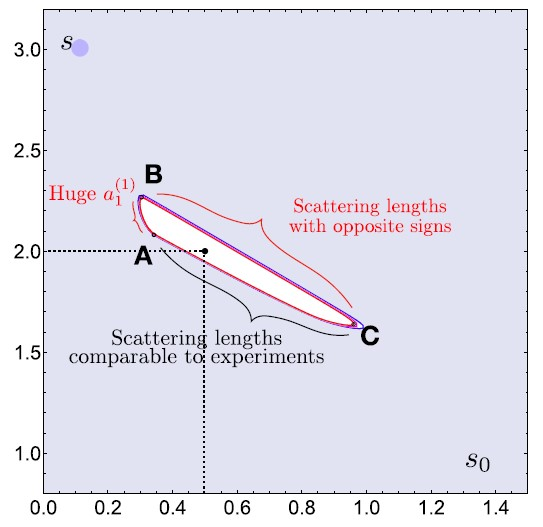
\includegraphics[width=5cm]{4.jpg}
\end{figure}
\end{frame}


\begin{frame}{Pion Bootstrap}
\framesubtitle{The Peninsula}
\begin{itemize}
\item At low energies the partial wave amplitude's real part can be expanded in its COM momentum $k=\sqrt{\frac{s-4}{4}}$ as \(\operatorname{Re}\left[\mathcal{T}_{\ell}^{(I)}\right]=k^{2 \ell}\left[a_{\ell}^{(I)}+b_{\ell}^{(I)} k^{2}+\mathcal{O}\left(k^{4}\right)\right] \) where $a_{\ell}^{(I)}$'s are called scattering lengths and $b_{\ell}^{(I)}$'s effective ranges.
 \item We now impose, apart from \textbf{all the conditions imposed in Lake}, the experimental values of the scattering lengths i.e $\left|a_{0}^{(0)}-0.2196\right|<0.034$, $\left|a_{1}^{(1)}-0.038\right|<0.002$ and $\left|a_{0}^{(2)}-(-0.0444)\right|<0.0012$ and repeating the same process, we obtain the \textbf{Pion Peninsula}.
\begin{figure}
    \centering
    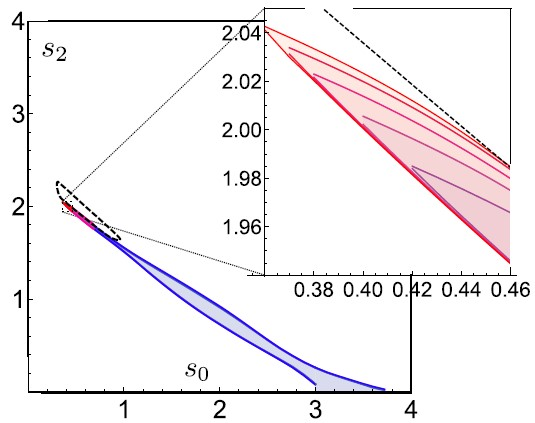
\includegraphics[width=5cm]{6.jpg}
\end{figure}
\end{itemize}
\end{frame}








\begin{frame}{Pion Bootstrap}
\framesubtitle{Analyticity in Mandelstram Plane \footnote[frame]{A.V.Manohar and V.Mateu,"Dispersion Relation Bounds for $\pi \pi$ Scattering" Phys. Rev. D 77, 094019 (2008)}}
\begin{itemize}
\item  $T^{*}(s+i \epsilon)=T(s-i \epsilon) \Rightarrow  T(s+i \epsilon)-T(s-i \epsilon)=2 i \operatorname{Im} T(s+i \epsilon) \neq 0$.\\Non-analyticity for $s \geq 4m^{2}$ will translate into crossed channels to give\\\textbf{Analyticity for  $s,t \leq 4m^{2}, s+t \geq 0$}
\item In complex $s$-plane with neighbourhood (in $s$) being analytic and $t<4m^{2}$ has branch cuts are at $s>4m^{2}$ and $s<-t$ and the following contour can be used to write (if contour at infinity vanishes which is the case for pion scattering with $n=2$)
\[\frac{d^{n}}{d s^{n}} T^{I}(s, t)=\frac{n !}{\pi} \int_{4 m^{2}}^{\infty} dx\left[\frac{\delta^{I I^{\prime}}}{(x-s)^{n+1}}\right. \left.+(-1)^{n} \frac{C_{u}^{I I^{\prime}}}{(x-u)^{n+1}}\right] \operatorname{Im} T^{I^{\prime}}(x+i \epsilon, t)\]
\begin{figure}[H]
  \centering
  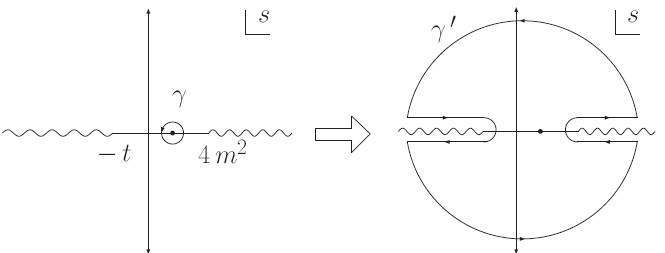
\includegraphics[width=6cm]{9.jpg}
\end{figure}
with $T^{I}(s, t) =C_{u}^{I I^{\prime}} T^{I^{\prime}}(u, t)$
\end{itemize}
\end{frame}



\begin{frame}{Pion Bootstrap}
\framesubtitle{Fixed $t$ dispersion relation}
\begin{itemize}
\item It can be shown that \textbf{$\operatorname{Im} T^{I}(s, t)>0$ for $t>0$} and $t>0$ along with $s,t<4m^{2}, s+t>0$ defines a region $\mathcal{A}$
\begin{figure}[H]
  \centering
  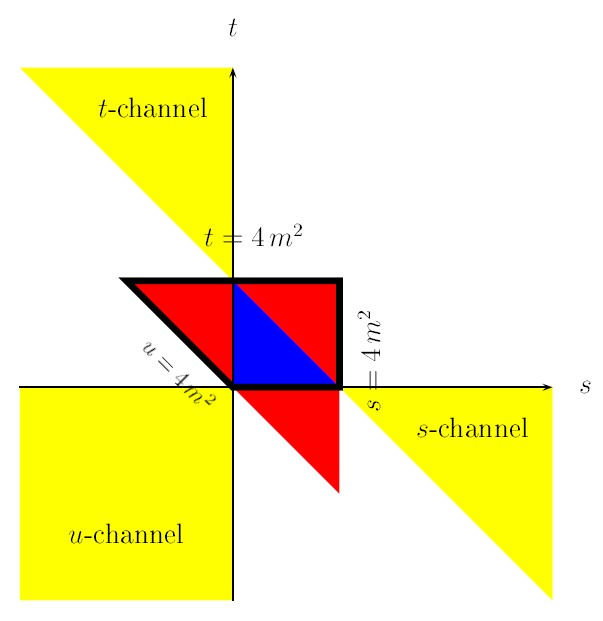
\includegraphics[width=4cm]{10.jpg}
\end{figure}
\item For the 3 scattering amplitudes $T=\sum a_{I} T^{I}$ has $a_{I} \geq 0$ and $b_{J}=\sum_{I} a_{I} C_{u}^{I J} \geq 0$ and
\begin{equation*}
    \begin{split}
\frac{d^{2}}{ds^{2}} T\left(\pi^{0} \pi^{0} \rightarrow \pi^{0} \pi^{0}\right)[(s, t) \in \mathcal{A}] \geq &0\qquad
\frac{d^{2}}{d s^{2}} T\left(\pi^{+} \pi^{0} \rightarrow \pi^{+} \pi^{0}\right)[(s, t) \in \mathcal{A}] \geq 0 \\
\frac{d^{2}}{d s^{2}} T\left(\pi^{+} \pi^{+} \rightarrow \pi^{+} \pi^{+}\right)[(s, t) \in \mathcal{A}] \geq &0
 \end{split}
    \end{equation*}
\end{itemize}
\end{frame}



\begin{frame}{Pion Bootstrap}
\framesubtitle{S,D-wave Inequalities}
\begin{itemize}
\item Now using $a_{\ell}^{I}=\lim _{s \rightarrow 4 m^{2}} \frac{T_{\ell}^{I}(s)}{\left(\frac{s}{4}-m^{2}\right)^{\ell}}$ and going through few steps, \[\left.\frac{d^{2} T^{I}\left(s, 4 m^{2}\right)}{d s^{2}}\right|_{s=0}=\frac{120}{32} C_{t}^{I J} a_{2}^{J}\geq 0  \qquad  I=0,1,2 \quad (0,4m^{2})\in\mathcal{A}\] 
where $T^{I}(s, t) =C_{t}^{I I^{\prime}} T^{I^{\prime}}(t, s)$
\item \textbf{D-wave Inequalities: }$a_{2}^{0}+2 a_{2}^{2} \geq 0, \quad a_{2}^{0}-a_{2}^{2} \geq 0$. Additionally choosing $a_{2}^{(2)}\geq 0$ makes phenomenological values lie in allowed region.
\item Leading order $\chi PT$ values give [9] \textbf{S-wave Inequalitites: } $a_{0}^{(0)}+2 a_{0}^{(2)} \geq 0, \quad 2 a_{0}^{(0)}+a_{0}^{(2)} \geq 0, \quad a_{0}^{(0)}-a_{0}^{(2)} \geq 0, \quad a_{0}^{(2)} \leq 0$.
\end{itemize}
\end{frame}

\begin{frame}{Pion Bootstrap [9]\footnote[frame]{A. Bose, P. Haldar, A. Sinha, Pritish Sinha, S. S. Tiwari, "Relative entropy in scattering and the S-matrix bootstrap" arXiv:2006.12213}}
\framesubtitle{River}
\begin{itemize}
\item  Constraints in \textbf{Lake} plus \textbf{S and D-wave Inequalities} gives the \textbf{River}
\begin{figure}[H]
  \centering
  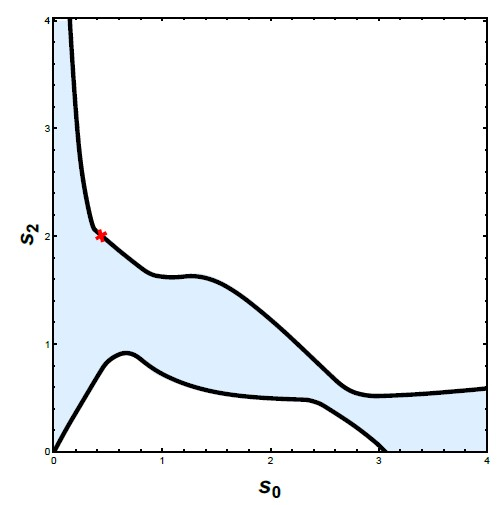
\includegraphics[width=6cm]{11.jpg}
\end{figure}
\end{itemize}
\end{frame}








\section{Bounds on Wilson Coefficients}

\begin{frame}{Crossing Symmetric Dispersion Relation  [6]\footnote[frame]{A. Sinha, A. Zahed, "Crossing Symmetric Dispersion Relations in QFTs"}}
\begin{itemize}
\item Dispersion relations used so far with fixed $t$ in complex $s$-plane is not crossing symmetric. 
\item Shifted variables $s_{1}=s-\frac{\mu}{3}, s_{2}=t-\frac{\mu}{3}, s_{3}=u-\frac{\mu}{3}$ and $s_{1}+s_{2}+s_{3}=0$. 
\item $s_{k}=a-\dfrac{a\left(z-z_{k}\right)^{3}}{z^{3}-1}, \quad k=1,2,3$ where $z_{k}$ are cube roots of unity. 
\item Amplitude can be written as $\overline{\mathcal{M}}(z, a)=\mathcal{M}\left(s_{1}, s_{2}\right)$ and for $-\frac{2\mu}{9}<a<0$, the branch cuts for $s,t,u\geq 4m^{2}=\mu$ become $s_{1},s_{2},s_{3}\geq \frac{8m^{2}}{3}=\frac{2\mu}{3}$ map to arcs in the unit circle in $z$-plane for fixed $a$ as shown
\begin{figure}[H]
  \centering
  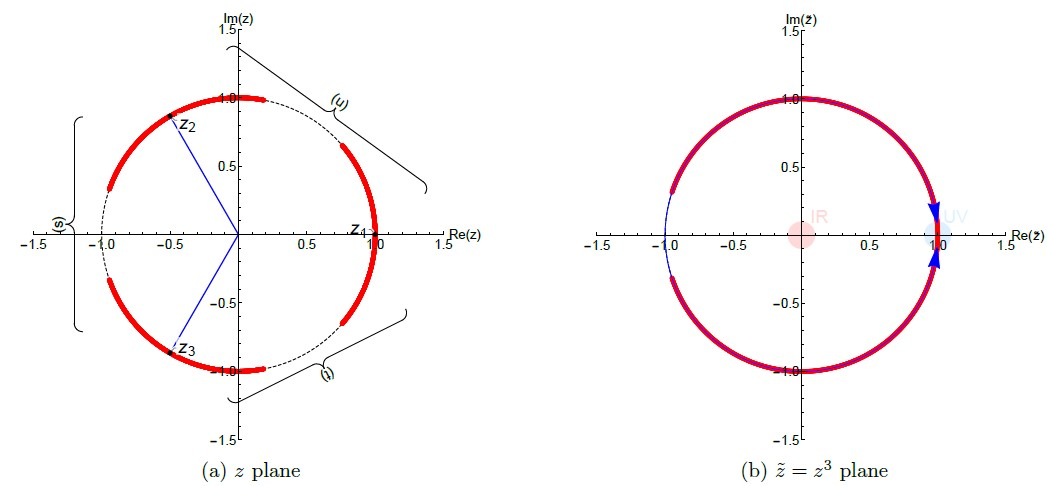
\includegraphics[width=7cm]{16.jpg}
  \caption{Cuts in $z$-plane and $\tilde z (=z^{3})$-plane}
  \label{fig:1}
\end{figure} 
\end{itemize}
\end{frame}

\begin{frame}{Crossing Symmetric Dispersion Relation}
\begin{itemize}
\item Defining $\tilde z (=z^{3})$, we can write the following completely symmetric dispersion relation for fixed $a$
\[\mathcal{M}(\tilde{z}, a)=\alpha_{0}+\frac{1}{\pi} \int_{\frac{2 \mu}{3}}^{\infty} \frac{d s_{1}^{\prime}}{s_{1}^{\prime}} \mathcal{A}\left(s_{1}^{\prime} ; s_{2}^{(+)}\left(s_{1}^{\prime}, a\right)\right) H\left(s_{1}^{\prime}, \tilde{z}\right)\]
where we have $s$-channel discontinuity as $\mathcal{A}_{1}\left(s_{1}, s_{2}\right) \equiv \lim _{\epsilon \rightarrow 0} \frac{1}{2 i}\left[\mathcal{M}\left(s_{1}+i \epsilon, s_{2}\right)-\mathcal{M}\left(s_{1}-i \epsilon, s_{2}\right)\right], \quad s \geqslant 2 \mu / 3$, $\alpha_{0}=$ $\mathcal{M}(z=0, a)$ and 
\begin{equation*}
    \begin{split}
&H\left(s_{1}^{\prime}, \tilde{z}\right)=\frac{27 a^{2} \tilde{z}\left(2 s_{1}^{\prime}-3 a\right)}{27 a^{3} \tilde{z}-27 a^{2} \tilde{z} s_{1}^{\prime}-(1-\tilde{z})^{2}\left(s_{1}^{\prime}\right)^{3}} \\
&s_{2}^{(+)}\left(s_{1}^{\prime}, a\right)=-\frac{s_{1}^{\prime}}{2}\left[1-\left(\frac{s_{1}^{\prime}+3 a}{s_{1}^{\prime}-a}\right)^{1 / 2}\right]
\end{split}
    \end{equation*}
\end{itemize}
\end{frame}


\begin{frame}{Univalence and de Branges' theorem [7]\footnote[frame]{P. Haldar, A. Sinha, A. Zahed, "Quantum field theory and the Bieberbach conjecture"}}
\begin{itemize}
\item We can write the kernel in the form \[H\left(s_{1}^{\prime}, \tilde{z}\right)=\frac{27 a^{2} \frac{\tilde z}{(1-\tilde z)^{2}}\left(2 s_{1}^{\prime}-3 a\right)}{27 a^{3}\frac{\tilde z}{(1-\tilde z)^{2}}-27 a^{2}\frac{\tilde z}{(1-\tilde z)^{2}} s_{1}^{\prime}-\left(s_{1}^{\prime}\right)^{3}}\]
\vspace{6pt}
\item We identify the repeatedly occuring factor as the \textbf{Koebe function} $k(z)=\frac{z}{(1-z)^{2}}=z+\sum_{p=2}^{\infty} p z^{p}$ which has a property called univalence. 
\vspace{6pt}
\item Univalence of a function $f$ implies $f(z)=f(w) \Rightarrow z=w$ in a domain $\mathds{D}$.
\vspace{6pt} 
\item Consider univalence of $g(z)=az+b z^{2}+c$ in unit disk $\mathds{D}=\{ z\left| |z|<1 \right. \}$. $g(z)-g(w)=az+b z^{2} -aw-b w^{2}=a(z-w)(1+\frac{b}{a}(z+w))$. For $g(z)=g(w)$ to imply necessarily that $z=w$, $|1+\frac{a}{b}(z+w)|\neq 0 \quad \forall |z|<1 \Rightarrow \left|\dfrac{a}{b}\right|<\dfrac{1}{2}$. 
\end{itemize}
\end{frame}


\begin{frame}{Univalence and de Branges' theorem}
\begin{itemize}
\item We shall take $a \in\left(-\frac{2 \mu}{9}, 0\right) \cup\left(0, \frac{4 \mu}{9}\right)$ and $s_{1} \in\left[\frac{2 \mu}{3}, \infty\right)$ and abbreviate this condition as $\blacklozenge$
\item For $\blacklozenge$, it can be shown that $\mathcal{A}\left(s_{1} ; s_{2}^{(+)}\left(s_{1}, a\right)\right) >0$ if $Im\left(\mathcal{T}^{(I)}_{l}\right) \geq 0  $ which is a weaker conditon than the non-linear $Im\left(\mathcal{T}^{(I)}_{l}\right) \geq \frac{\sqrt{s-4}}{\sqrt{s}} \left|\mathcal{T}^{(I)}_{l}\right|^{2}$
\item Expanding $H\left(s_{1}^{\prime}, \tilde{z}\right)=\sum_{n=0}^{\infty} \beta_{n}\left(a, s_{1}^{\prime}\right) \tilde{z}^{n}$, it can be deduced that $\beta_{0}=0,\;\;\beta_{1}<0$ in $\blacklozenge$
\item $F\left(\tilde{z} ; s_{1}, a\right)=\dfrac{H\left(\tilde{z} ; s_{1}, a\right)}{\beta_{1}\left(a, s_{1}\right)}=\tilde{z}+\sum_{n=2}^{\infty} \dfrac{\beta_{n}\left(a, s_{1}\right)}{\beta_{1}\left(a, s_{1}\right)} \tilde{z}^{n}$
\item $F$ has no singularities in the unit disk for $\blacklozenge$ and $F$ can be written as Mobius tranformation of Koebe function as \[F\left(\tilde{z} ; s_{1}, a\right)=k(\tilde{z})\left(1-\frac{27 a^{2}\left(a-s_{1}\right)}{s_{1}^{3}} k(\tilde{z})\right)^{-1}\] 
\item \textbf{Mobius transformations of Koebe functions are univalent}. Additionally, univalence of $F$ implies univalence of the kernel $H$.
\end{itemize}
\end{frame}


\begin{frame}{Univalence and de Branges' theorem}
\begin{itemize}
\item \textbf{de Branges' Theorem:- }If $f$ is a univalent function with $f(z)=z+\sum_{p=2}^{\infty} b_{p} z^{p}, \quad|z|<1$, then its coefficients satisfy \[\left|b_{n}\right| \leq n, \quad \forall n \geq 2\] with equality iff $f$ is a Koebe function.
\item Using de Brange's Theorem on $F$, $\left|\dfrac{\beta_{n}\left(a, s_{1}\right)}{\beta_{1}\left(a, s_{1}\right)}\right| \leq n, \quad n \geq 2$
\item $\mathcal{M}$, when written in terms of $s_{1}, s_{2}$, can be expanded in  $x=-\left( s_{1} s_{2} + s_{2} s_{3} + s_{3} s_{1} \right)=s_{1}^{2}+s_{2}^{2}+s_{1}s_{2} \text{ and } y=-s_{1} s_{2}s_{3}=s_{1}s_{2}(s_{1}+s_{2})$ as \[\mathcal{M}\left(s_{1}, s_{2}\right)=\sum_{p,q=0}^{\infty} W_{p, q} x^{p} y^{q}\]
\item $\mathcal{M}(\tilde{z}, a)=\sum_{n=0}^{\infty} \alpha_{n}(a) a^{2 n} \tilde{z}^{n}$
and using the transformation  
\[\alpha_{p}(a) a^{2 p}=\sum_{n=0}^{p} \sum_{m=0}^{n} W_{n-m, m} a^{m}(-1)^{p-n}(-27)^{n} a^{2 n}\left(\begin{array}{c}
-2 n \\
p-n
\end{array}\right)
\]
\end{itemize}
\end{frame}


\begin{frame}{Bounds on Wilson Coefficients}
Since both $\mathcal{M}$ and $H$ are expanded in $\tilde z$, we can write
\begin{equation*}
    \begin{split}
\left|\alpha_{n}(a) a^{2 n}\right|&=\frac{1}{\pi}\left|\int_{\frac{2 \mu}{3}}^{\infty} \frac{d s_{1}^{\prime}}{s_{1}^{\prime}} \mathcal{A}\left(s_{1}^{\prime} ; s_{2}^{(+)}\left(s_{1}^{\prime}, a\right)\right) \beta_{n}\left(a, s_{1}^{\prime}\right)\right|\\
&\leq \frac{1}{\pi} \int_{\frac{2 \mu}{3}}^{\infty} \frac{d s_{1}^{\prime}}{s_{1}^{\prime}}\left|\mathcal{A}\left(s_{1}^{\prime} ; s_{2}^{(+)}\left(s_{1}^{\prime}, a\right)\right) \beta_{n}\left(a, s_{1}^{\prime}\right)\right|\\
&\leq \frac{1}{\pi} \int_{\frac{2 \mu}{3}}^{\infty} \frac{d s_{1}^{\prime}}{s_{1}^{\prime}} \mathcal{A}\left(s_{1}^{\prime} ; s_{2}^{(+)}\left(s_{1}^{\prime}, a\right)\right) n\left|\beta_{1}\left(a, s_{1}^{\prime}\right)\right|\\
&=n\left(-\alpha_{1}(a) a^{2}\right)=n\left|\alpha_{1}(a) a^{2}\right|
\end{split}
    \end{equation*}
$\left|\dfrac{\alpha_{n}(a) a^{2 n}}{\alpha_{1}(a) a^{2}}\right| \leq n$ for $n\geq 2$ for $\blacklozenge$ \\
For $n=2$ gives $-2 \leq 2-\dfrac{27 a^{2}\left(a\left(a W_{0,2}+W_{1,1}\right)+W_{2,0}\right)}{a W_{0,1}+W_{1,0}} \leq 2$\\
By not allowing denominator to be $0$, for $-\dfrac{2 \mu}{9}<a<\dfrac{4 \mu}{9}$, we get the first bound $-\dfrac{9}{16}<\dfrac{W_{0,1}}{W_{1,0}}<\dfrac{9}{8}$. The other bounds are obtained in [8]\footnote[frame]{A. Sinha, Prashanth Raman, "QFT,EFT and GFT" (Upcoming)}
\end{frame}


\begin{frame}{Results}
SDPB outputs the parameters and tha can be used to write down the S-matrices/scattering ampltudes at the boundaries of Lake, Peninsula, River. From those, the ratios $\dfrac{W_{p,q}}{W_{1,0}}$ were extracted (the denominator has been dropped in the table shown below). The River provided all but two of the overall min/max. So its plots for $\frac{W_{p,q}}{W_{1,0}}$ vs $s_{0}$ for points on its upper and lower boundaries are shown later.
\begin{figure}[H]
    \centering
    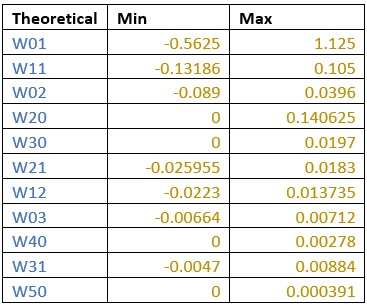
\includegraphics[width=5cm]{TabTh.jpg} 
	\caption{Theoretical Bounds. From [8]\footnote[frame]{A. Sinha, Prashanth Raman, "QFT,EFT and GFT"}}
\end{figure}
\end{frame}


\begin{frame}{Results}
 The overall minima and maxima for each ratio are plotted with the theoretical bounds.
\begin{figure}[H]
    \centering
    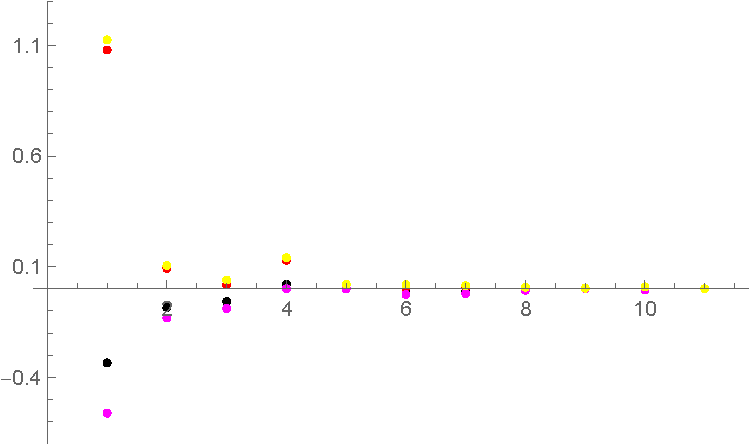
\includegraphics[width=10cm]{Plot1.pdf} 
\end{figure}
\end{frame}

\begin{frame}{Results}
\begin{figure}[H]
    \centering
    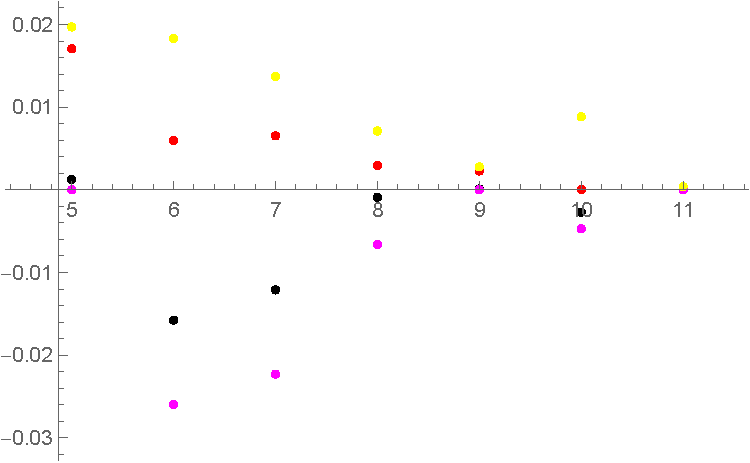
\includegraphics[width=10cm]{Plot2.pdf} 
\end{figure}
\end{frame}

\begin{frame}{Results}
\begin{figure}[H]
    \centering
    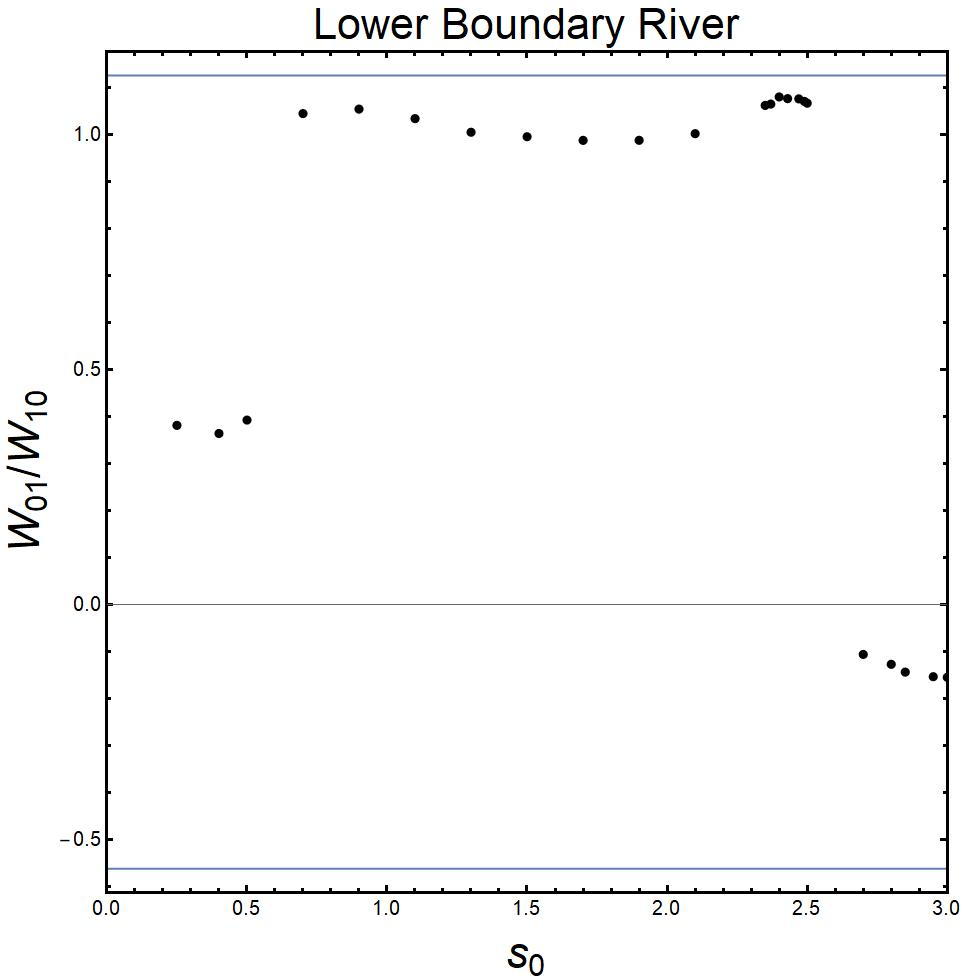
\includegraphics[width=3.5cm]{L01.jpg} 
    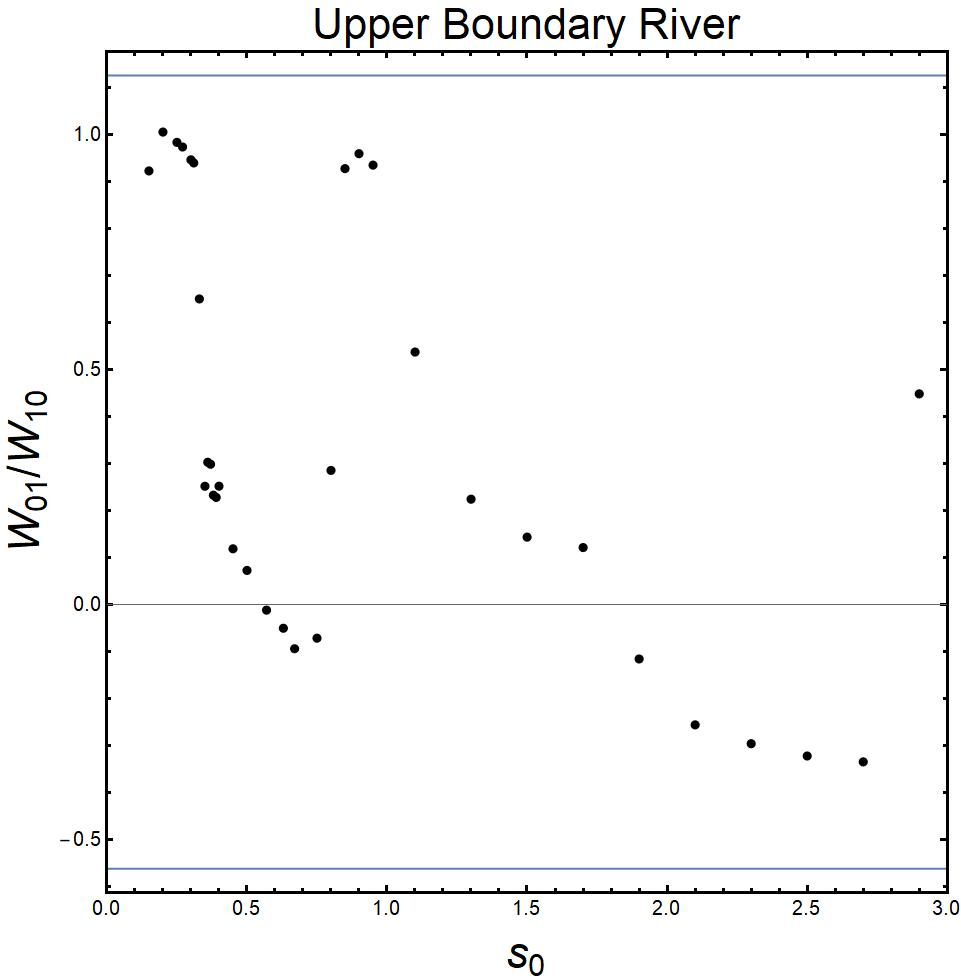
\includegraphics[width=3.5cm]{U01.jpg} 
\end{figure}
\begin{figure}[H]
    \centering
    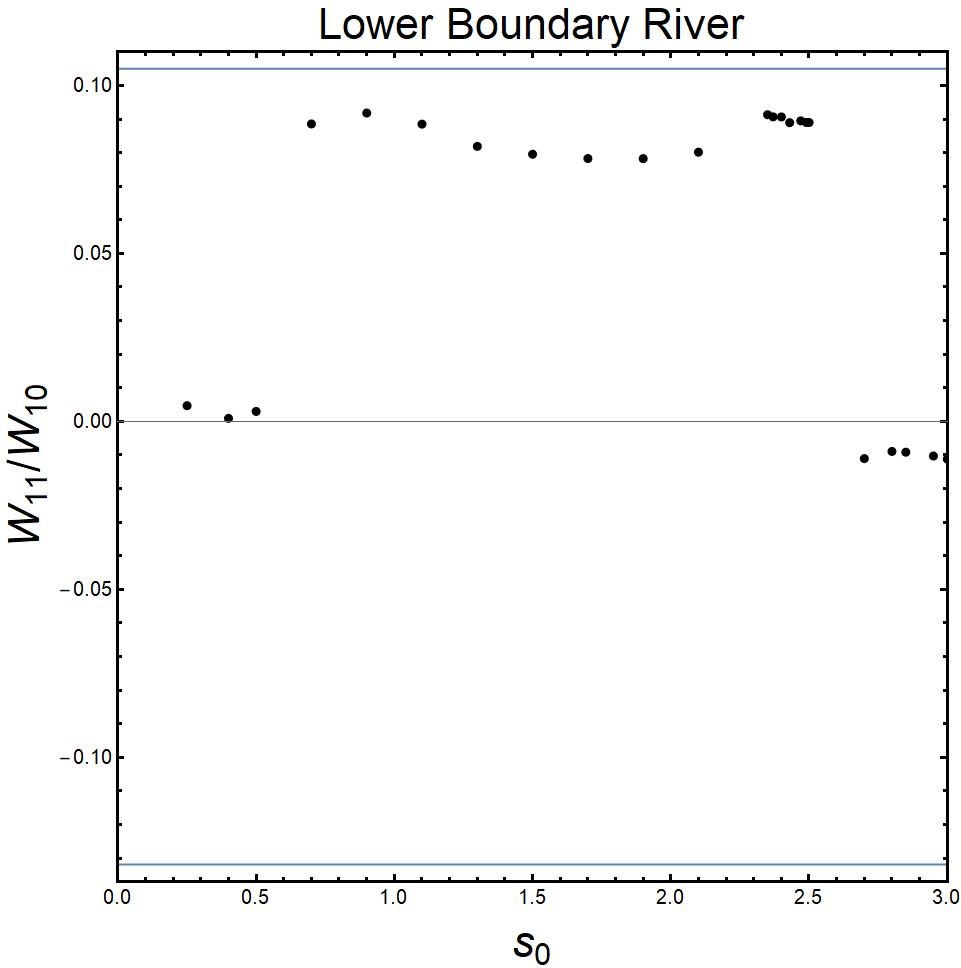
\includegraphics[width=3.5cm]{L11.jpg}
    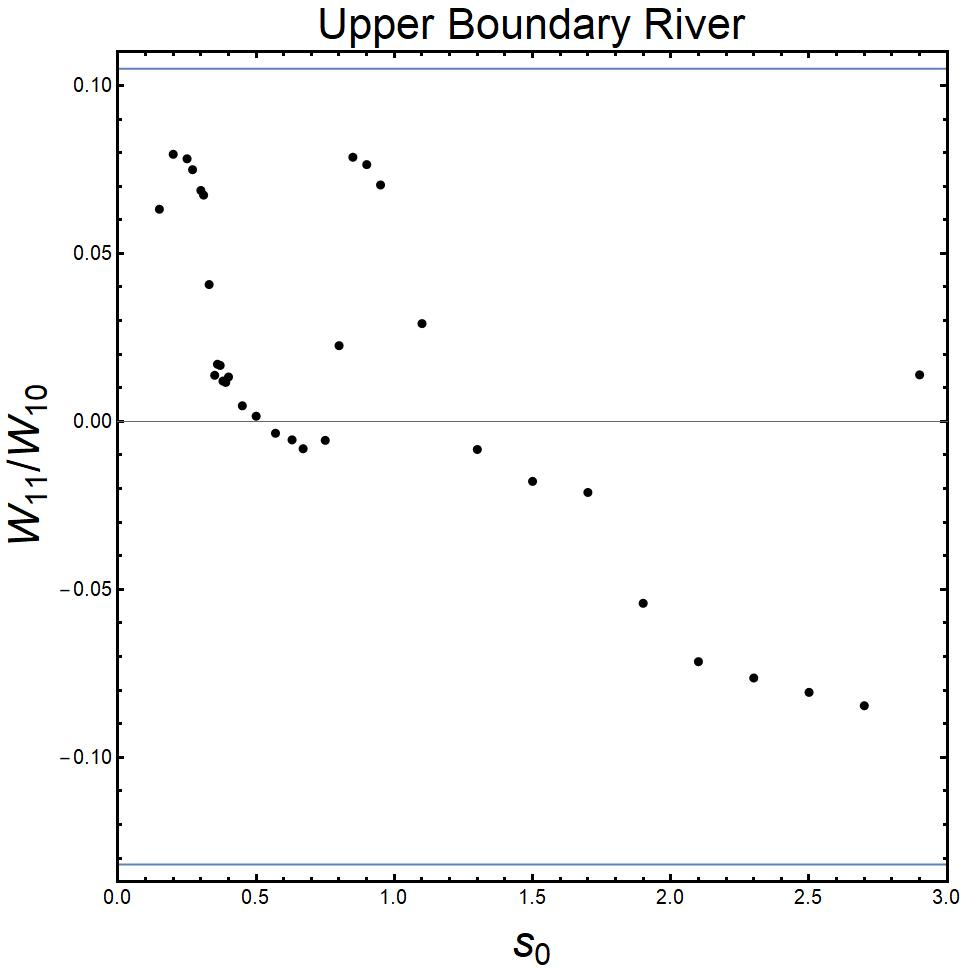
\includegraphics[width=3.5cm]{U11.jpg} 
\end{figure}
\end{frame}

\begin{frame}{Results}
\begin{figure}[H]
    \centering
    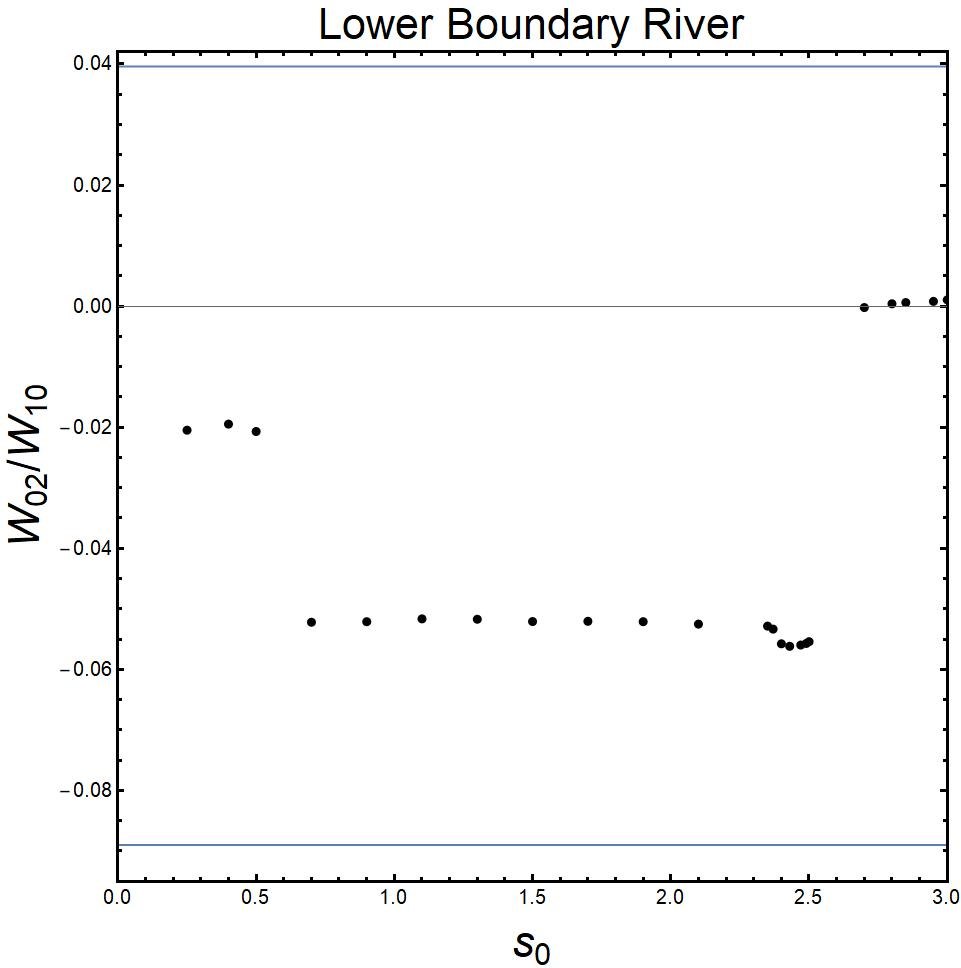
\includegraphics[width=3.5cm]{L02.jpg} 
    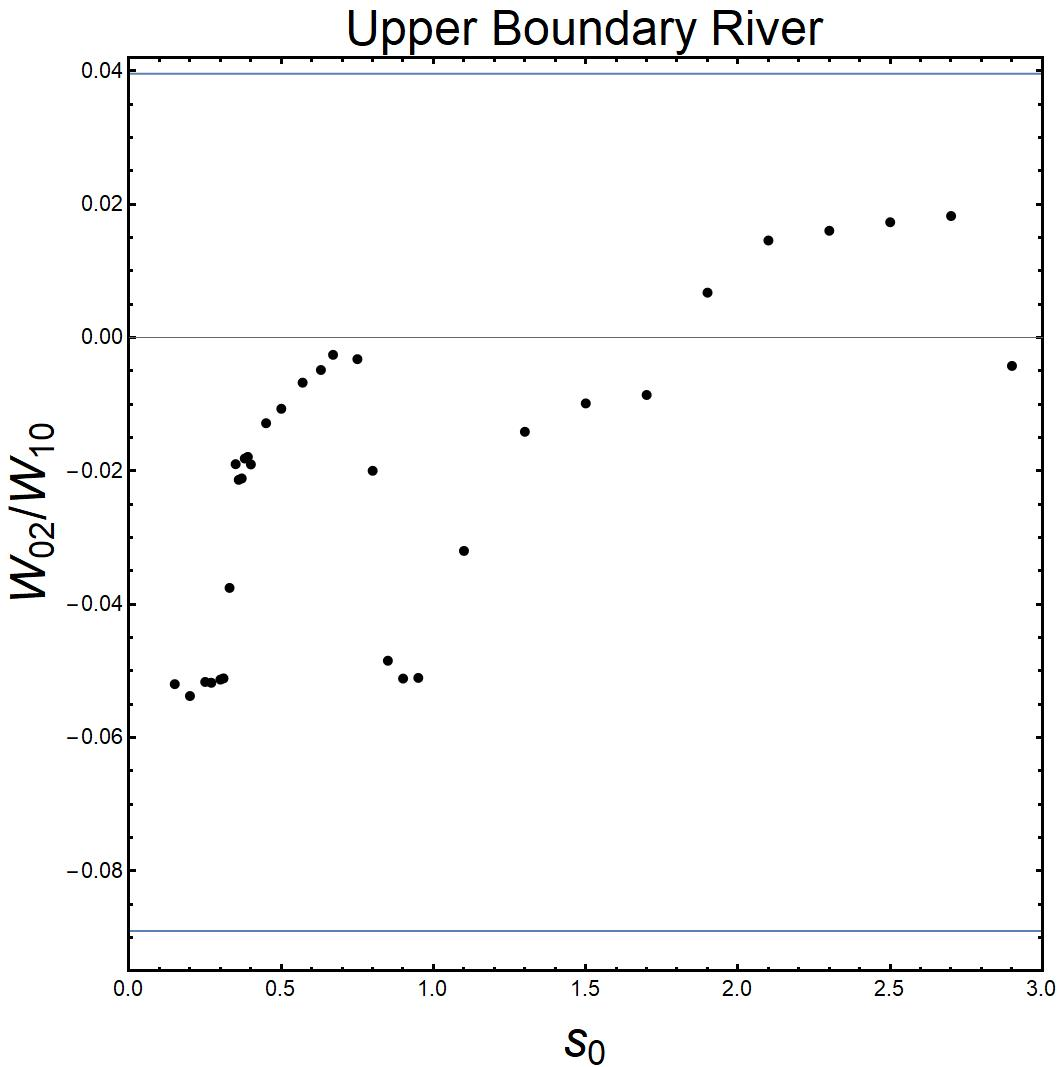
\includegraphics[width=3.5cm]{U02.jpg} 
\end{figure}
\begin{figure}[H]
    \centering
    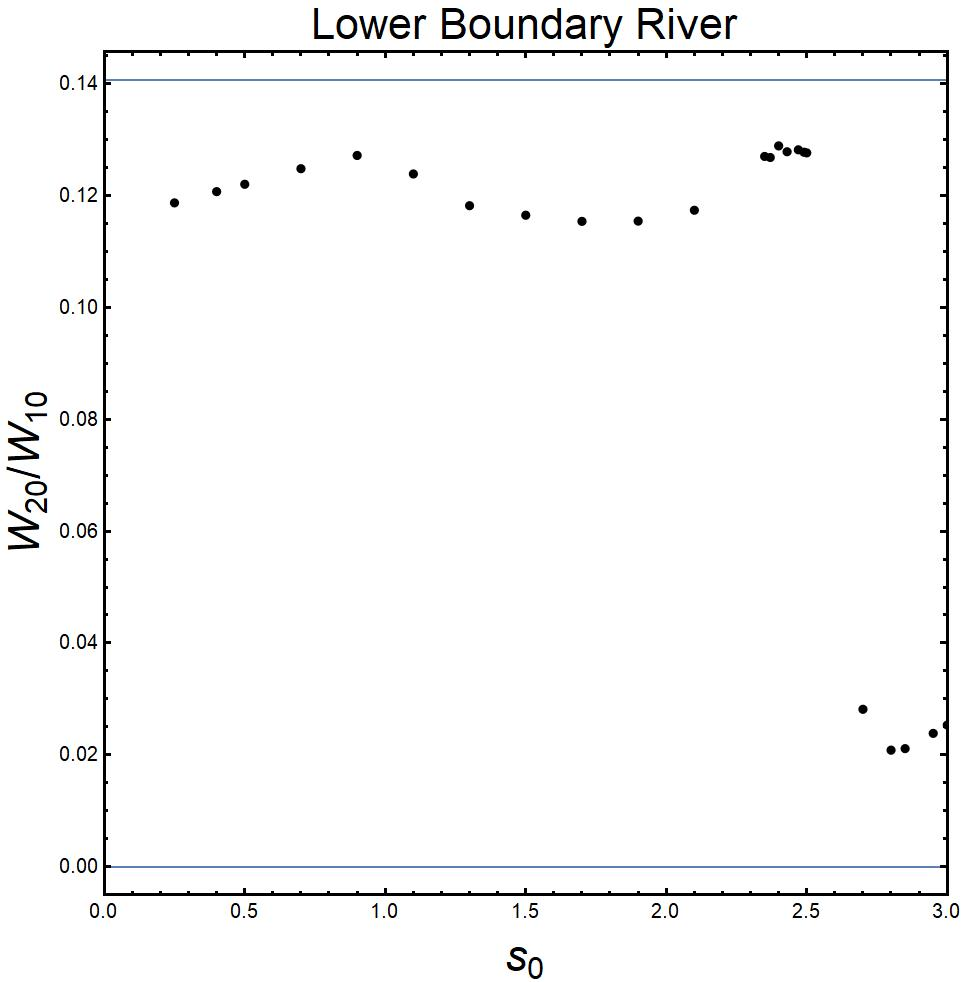
\includegraphics[width=3.5cm]{L20.jpg}
    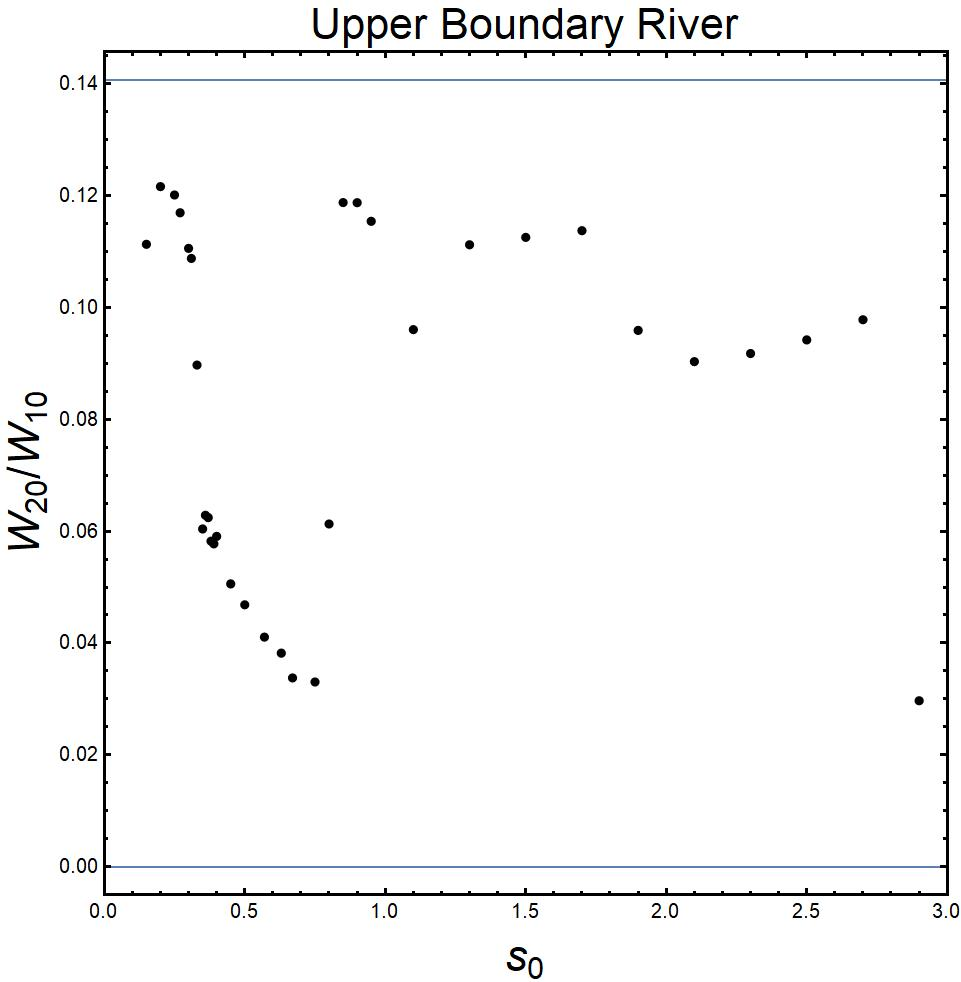
\includegraphics[width=3.5cm]{U20.jpg} 
\end{figure}
\end{frame}

\begin{frame}{Results}
\begin{figure}[H]
    \centering
    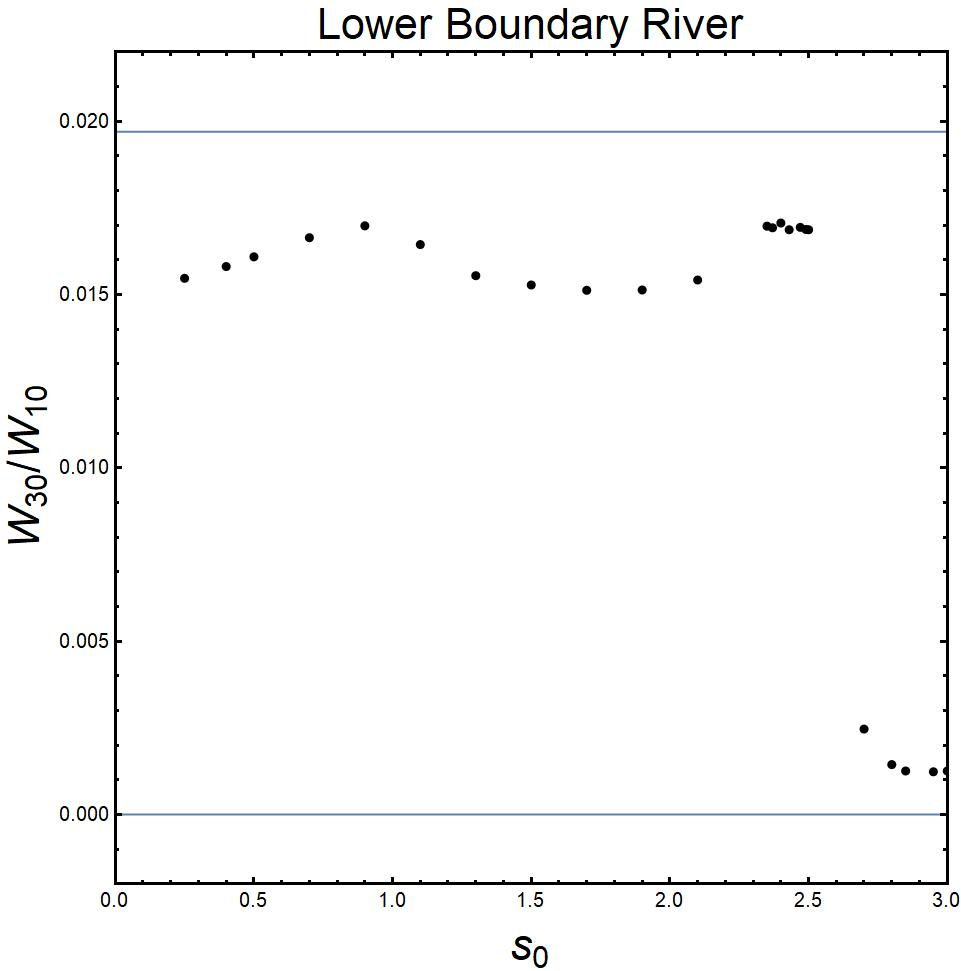
\includegraphics[width=3.5cm]{L30.jpg} 
    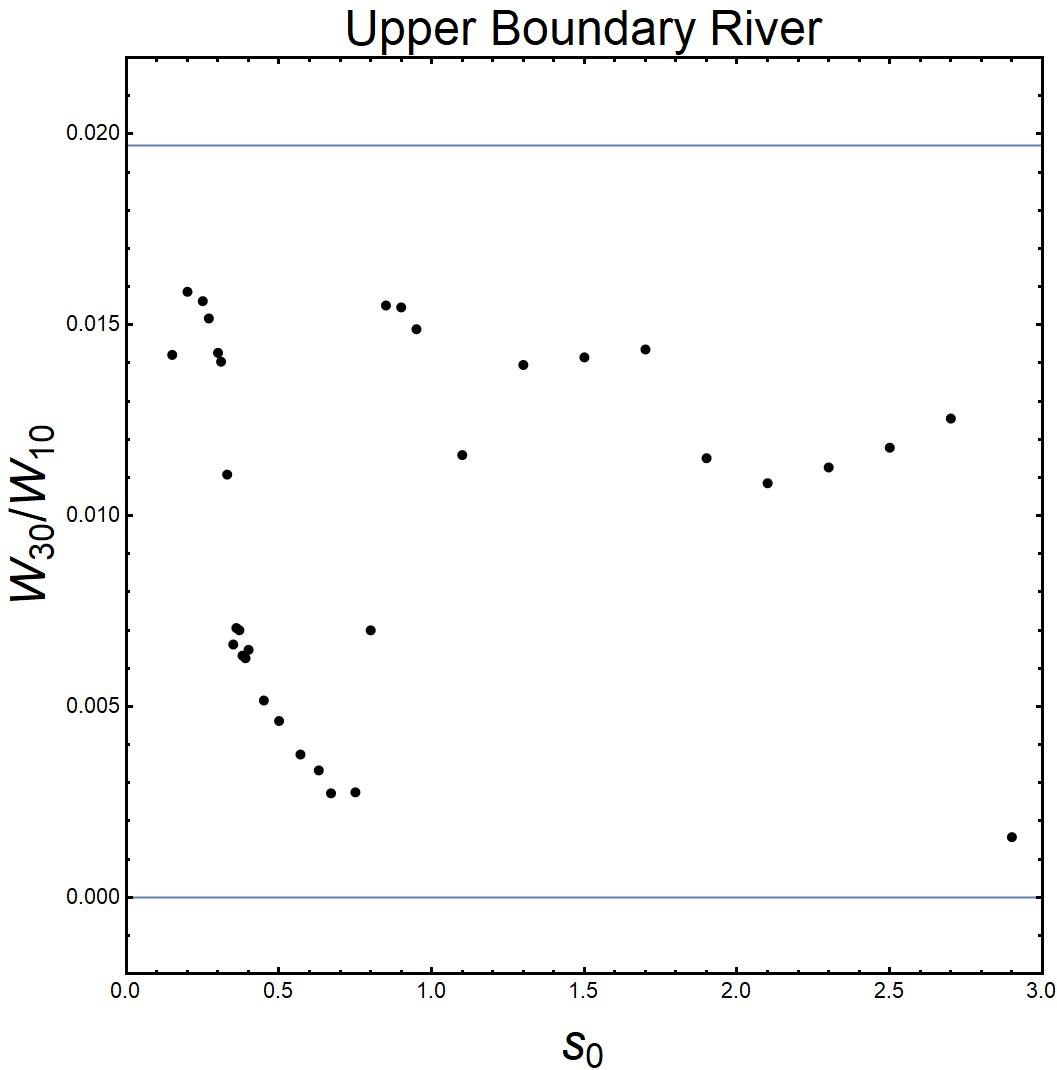
\includegraphics[width=3.5cm]{U30.jpg} 
\end{figure}
\begin{figure}[H]
    \centering
    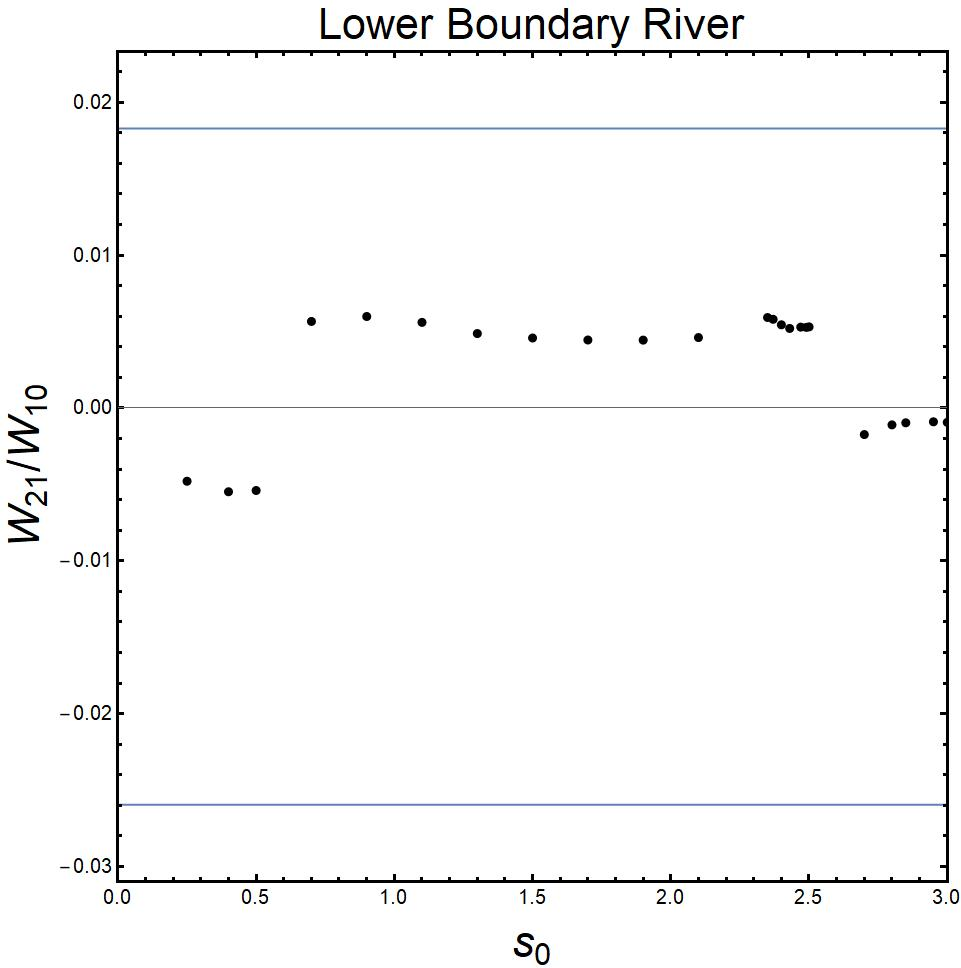
\includegraphics[width=3.5cm]{L21.jpg}
    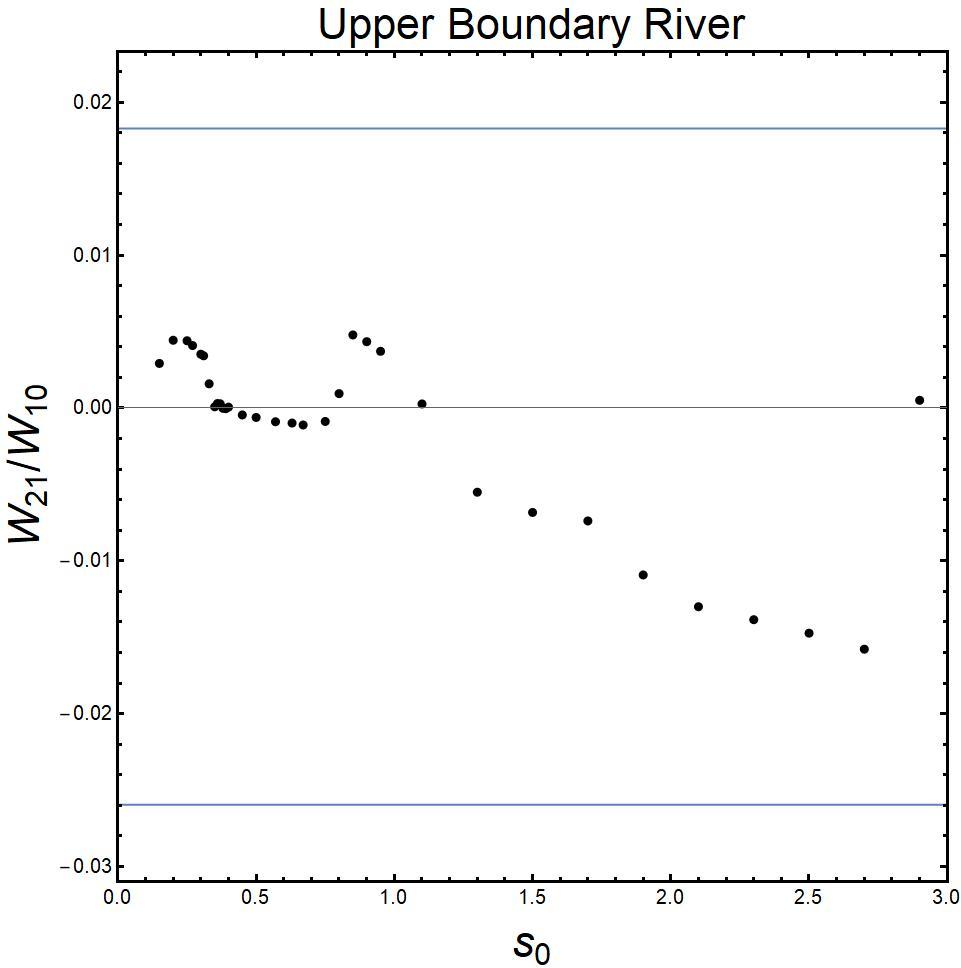
\includegraphics[width=3.5cm]{U21.jpg} 
\end{figure}
\end{frame}



\begin{frame}{Results}
\begin{figure}[H]
    \centering
    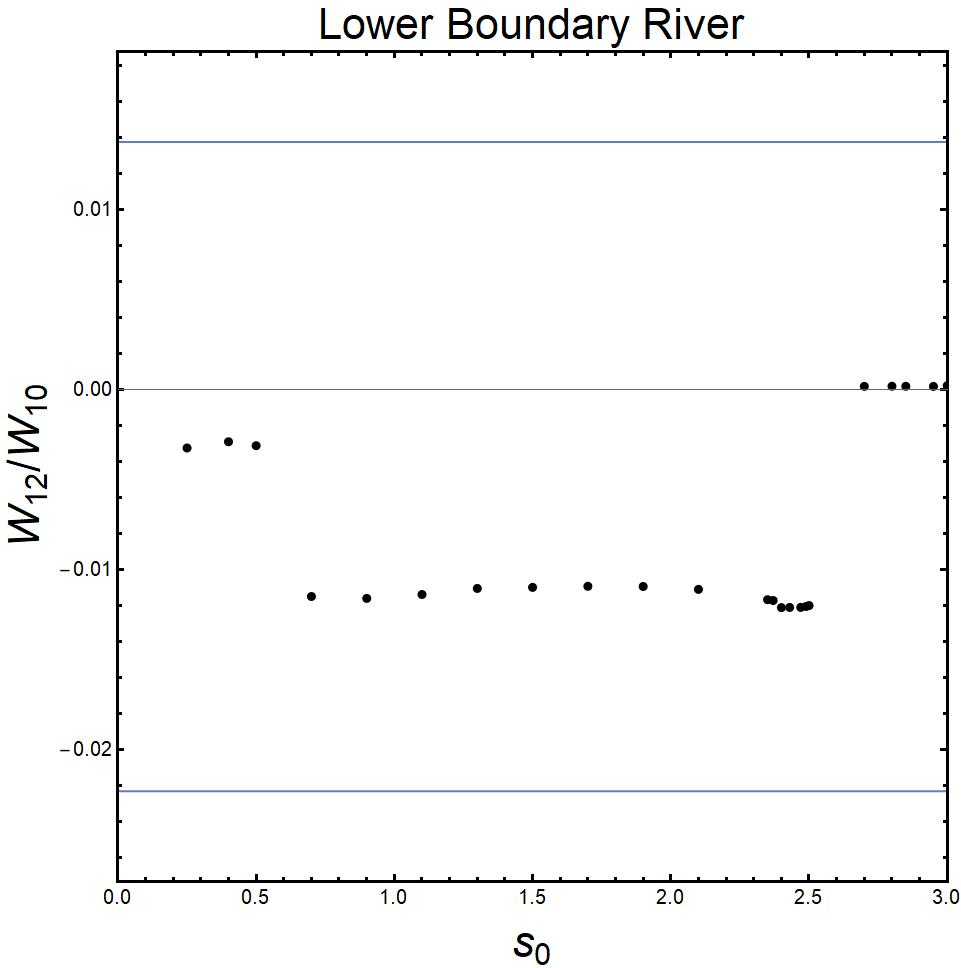
\includegraphics[width=3.5cm]{L12.jpg} 
    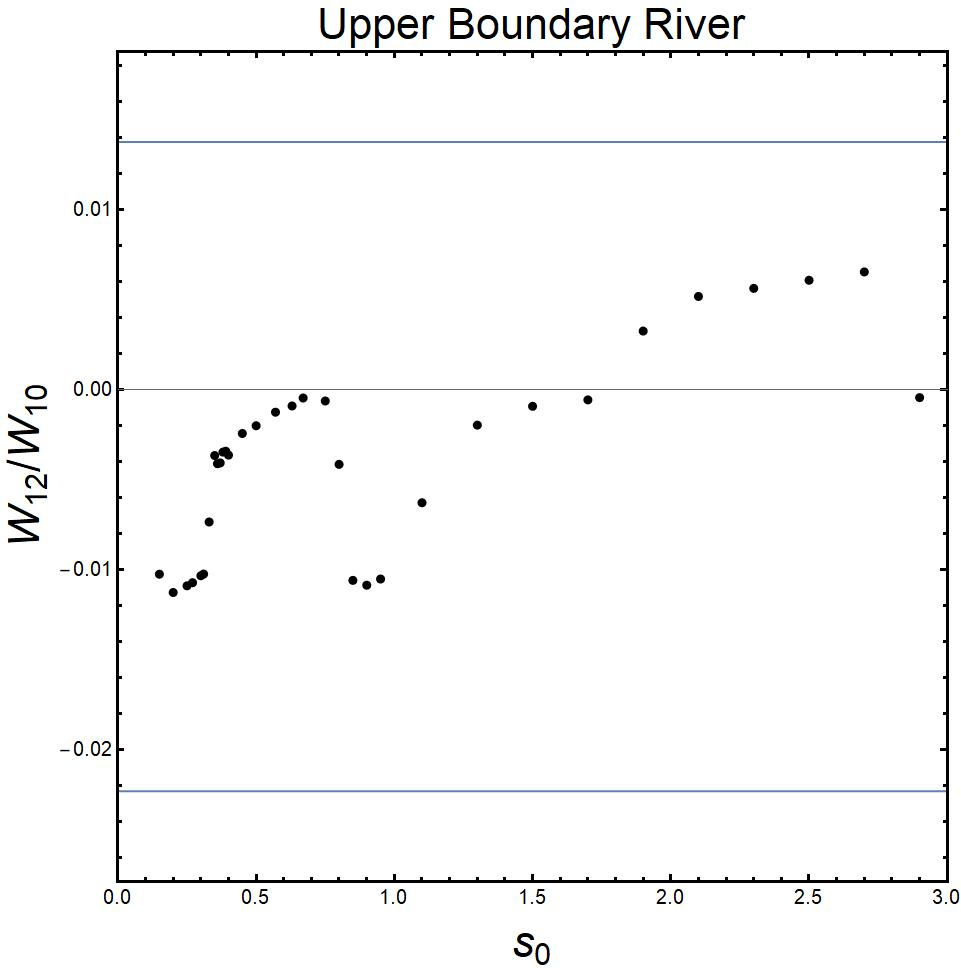
\includegraphics[width=3.5cm]{U12.jpg} 
\end{figure}
\begin{figure}[H]
    \centering
    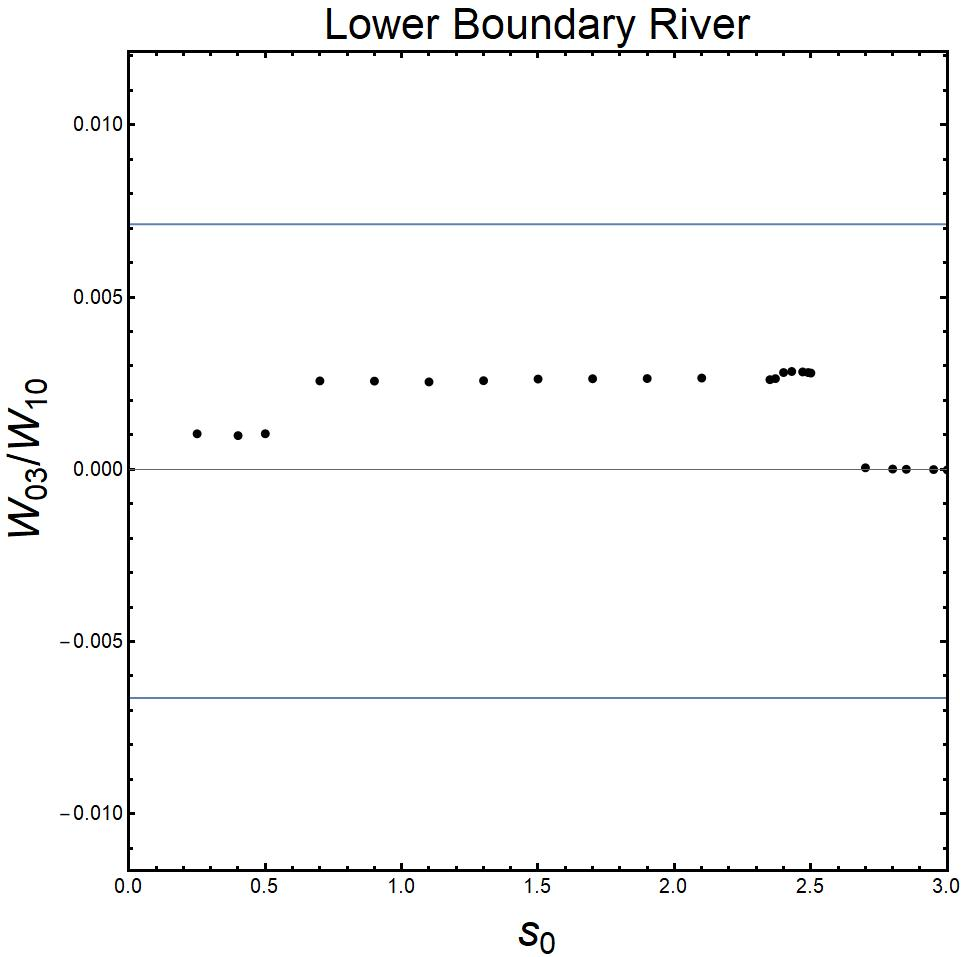
\includegraphics[width=3.5cm]{L03.jpg}
    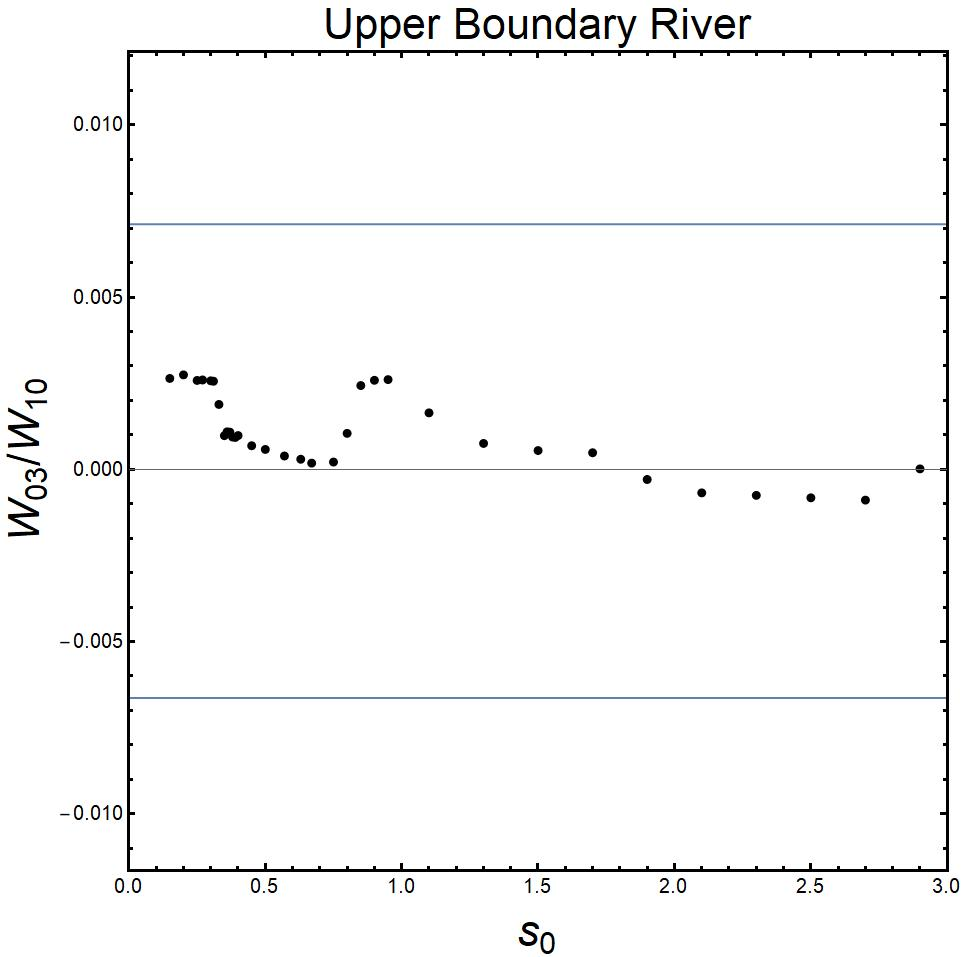
\includegraphics[width=3.5cm]{U03.jpg} 
\end{figure}
\end{frame}

\begin{frame}{Results}
\begin{figure}[H]
    \centering
    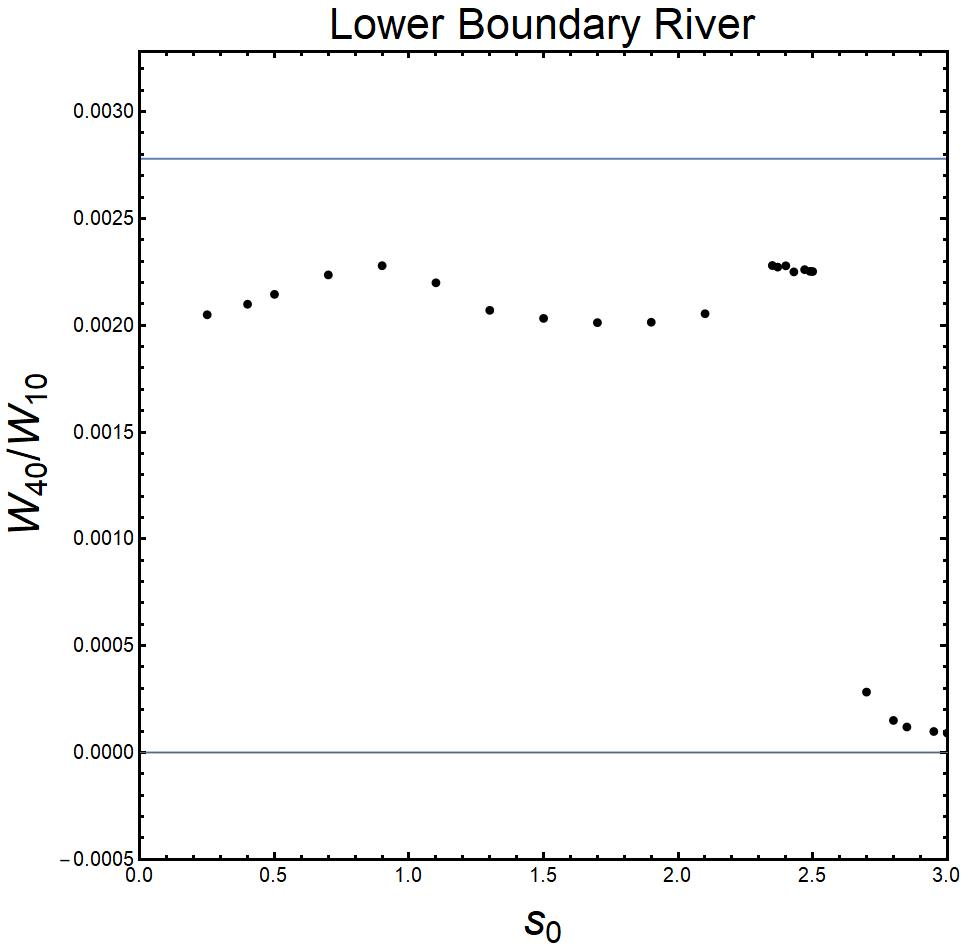
\includegraphics[width=3.5cm]{L40.jpg} 
    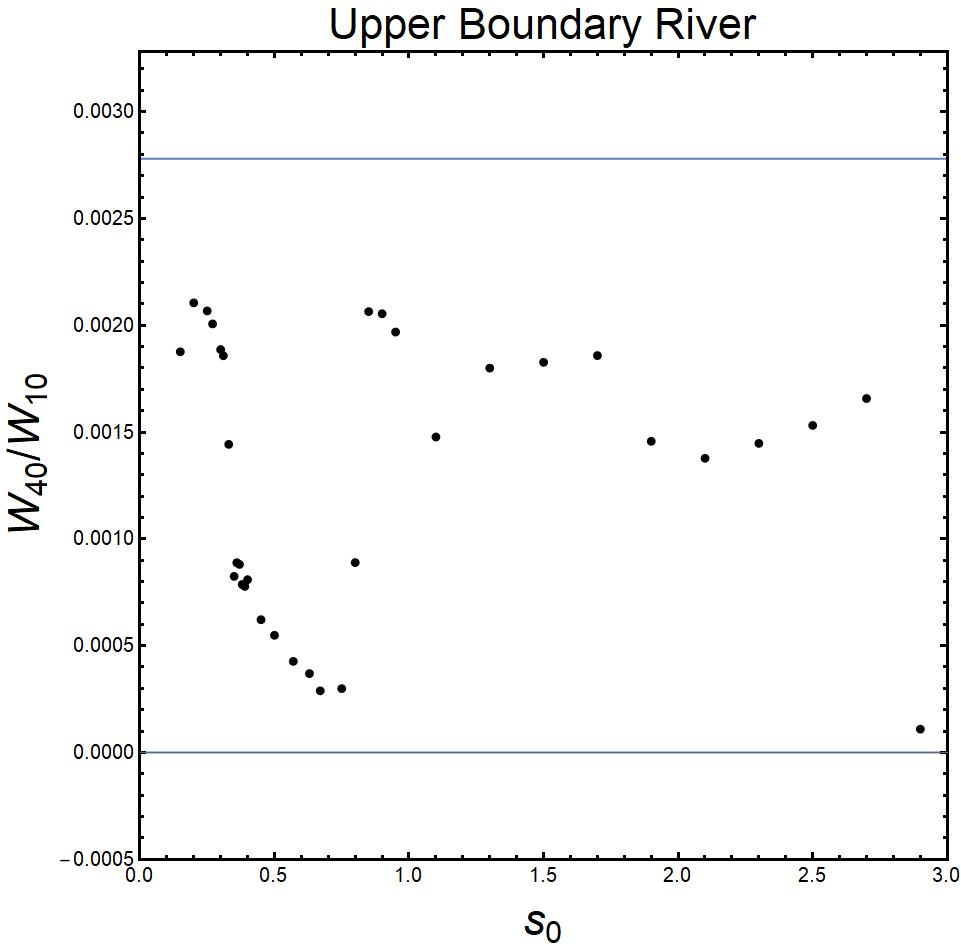
\includegraphics[width=3.5cm]{U40.jpg} 
\end{figure}
\begin{figure}[H]
    \centering
    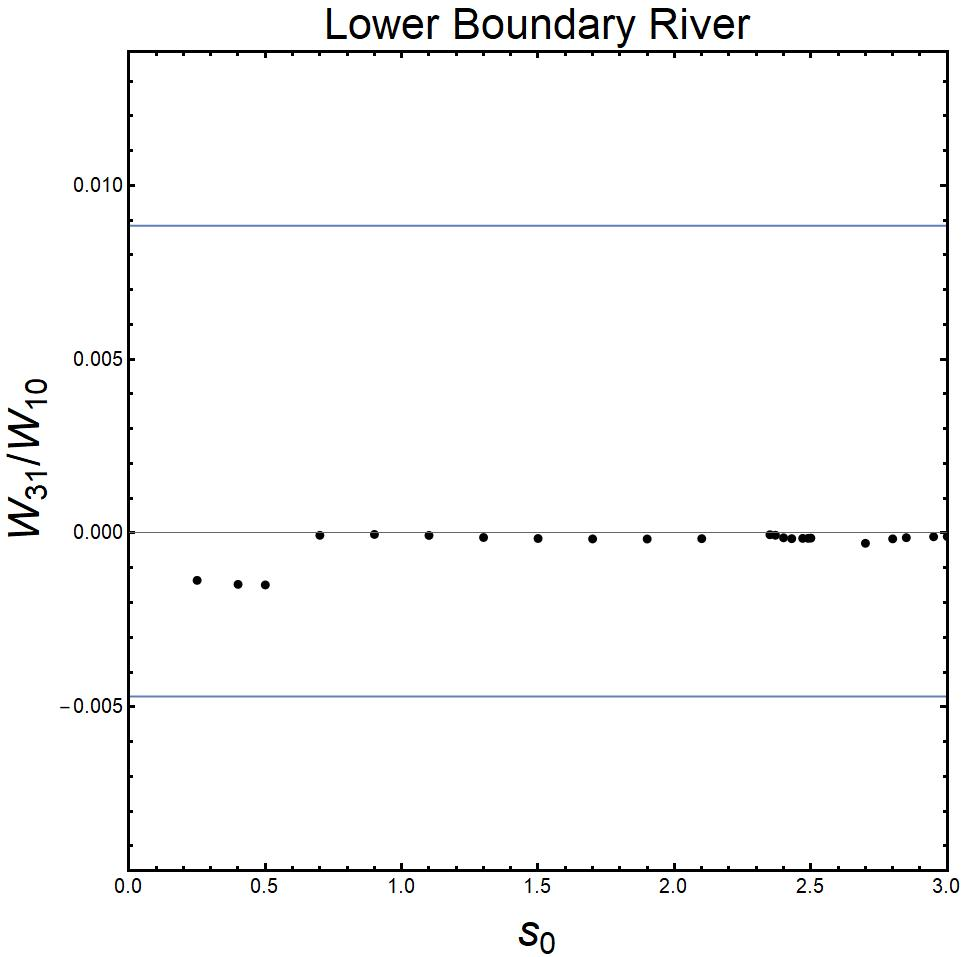
\includegraphics[width=3.5cm]{L31.jpg}
    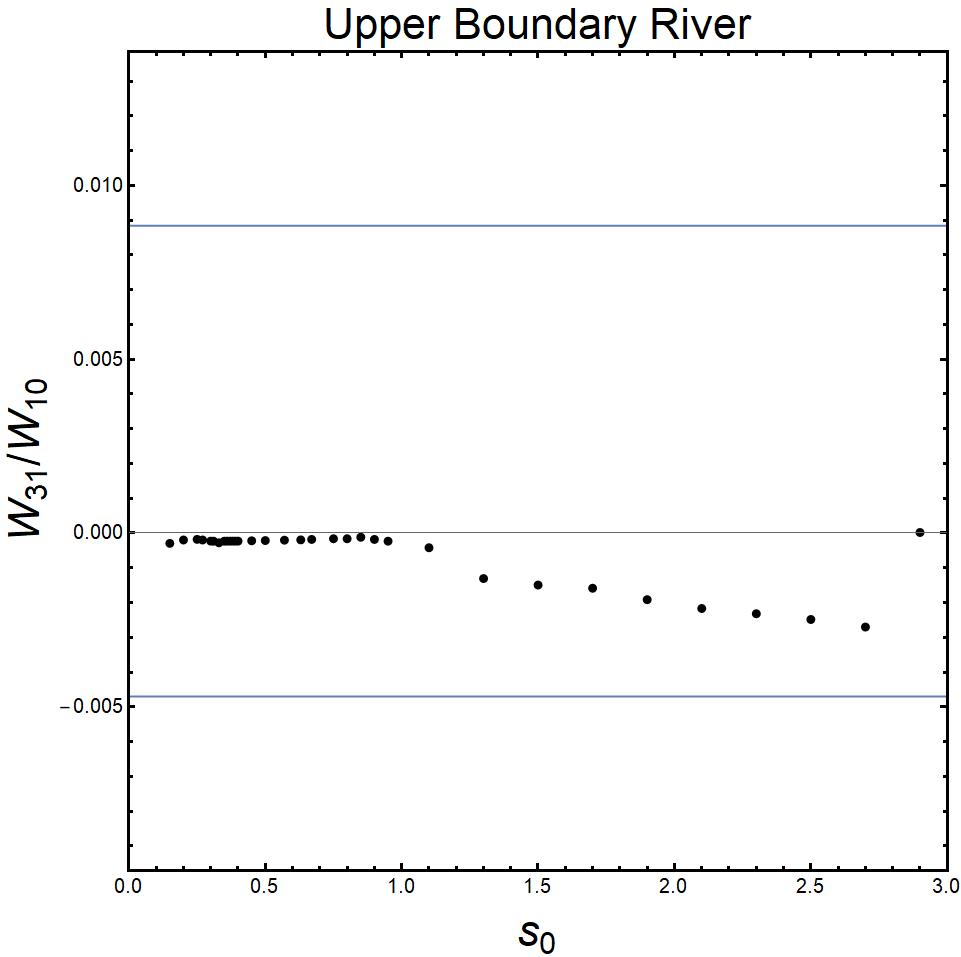
\includegraphics[width=3.5cm]{U31.jpg} 
\end{figure}
\end{frame}

\begin{frame}{Results}
\begin{figure}[H]
    \centering
    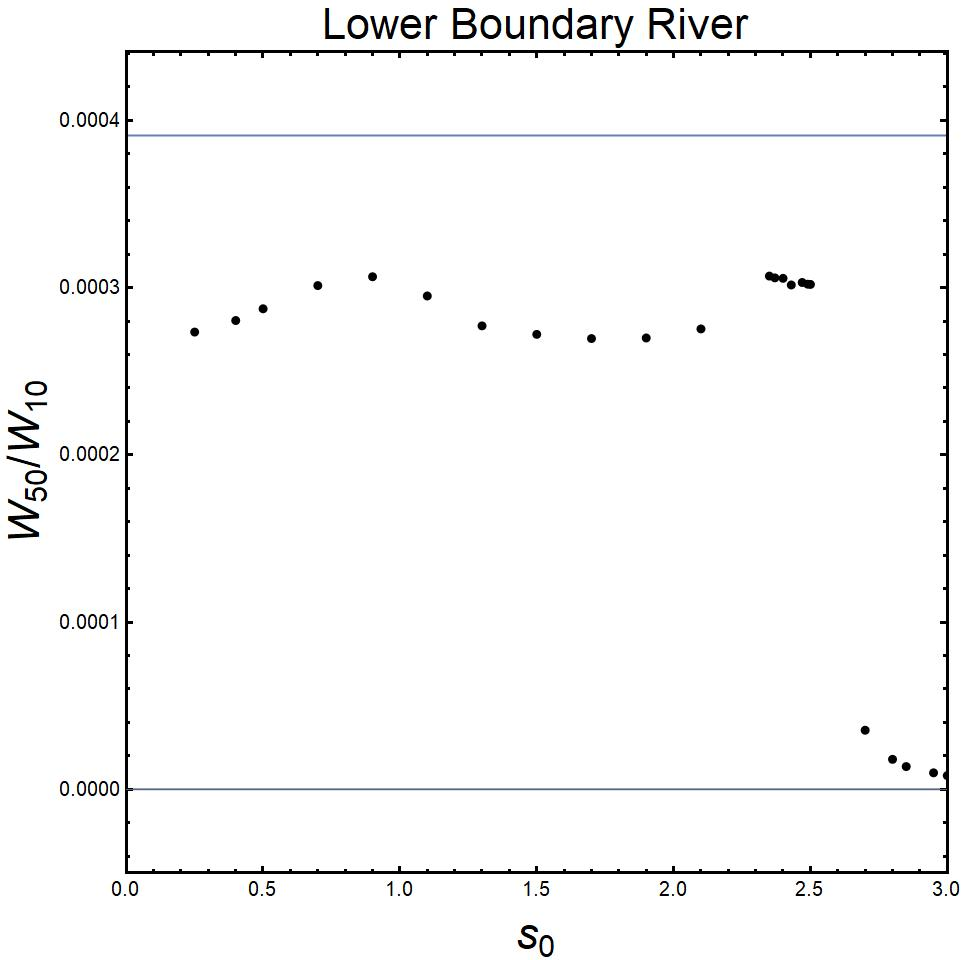
\includegraphics[width=5.5cm]{L50.jpg} 
    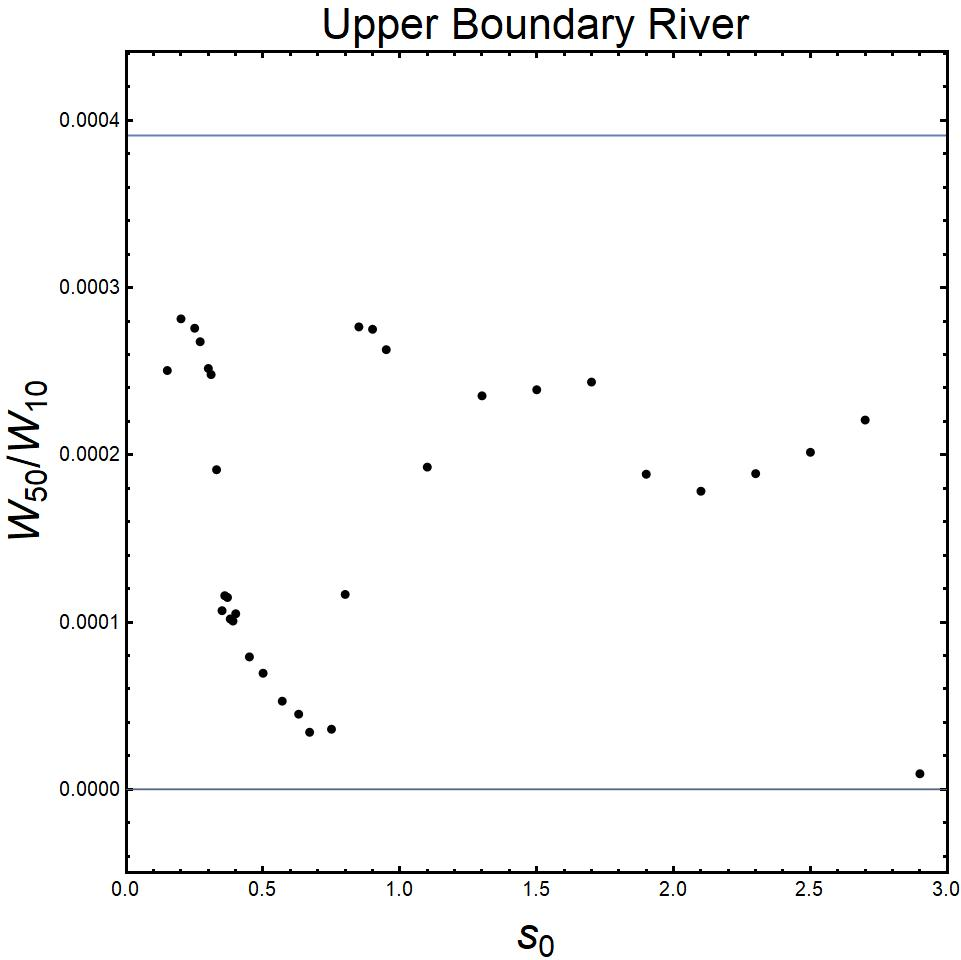
\includegraphics[width=5.5cm]{U50.jpg} 
\end{figure}

\end{frame}






\section{String Bootstrap}
\begin{frame}{String Bootstrap [4] \footnote[frame]{A. Guerrieri, J. Penedones, P. Vieira, "Where is String Theory?" arxiv.org:2102.02847}}
\framesubtitle{Ansatz}
\begin{itemize}
\item Constrain Wilson coeff. at $\mathcal{O}(s^{0})$, $\alpha$ in $\dfrac{T(s, t, u)}{8 \pi G_{N}}=s^{4}\left(\frac{1}{s t u}+\alpha \ell_{P}^{6}+O(s)\right)$.
\item Using a transformation to map the cut Mandelstram plane to a unit disk $\rho_{s} = \frac{\sqrt{s_{0}}-\sqrt{-s}}{\sqrt{s_{0}}+\sqrt{-s}}$, we write a crossing symmetric ansatz symmetric in all Mandelstram variables \[\frac{T}{8 \pi G_{N}}=s^{4}\left(\frac{1}{s t u}+\prod_{A=s, t, u}\left(\rho_{A}+1\right)^{2} \sum_{a+b+c \leq N}^{\prime} \alpha_{(a b c)} \rho_{s}^{a} \rho_{t}^{b} \rho_{u}^{c}\right)\]
The factor $\prod_{A=s, t, u}\left(\rho_{A}+1\right)^{2} \sim \frac{1}{s t u}$ keeps that part of the ansatz in control at high energies.
\item In 9+1 dim $P_{l}^{(9)}(x)=\frac{1}{3\cdot 2^{18}\cdot \pi^{4}} \frac{C_{l}^{7/2}(x)}{C_{l}^{7/2}(1)}$ can be used to write for massless case
\begin{equation*}
    \begin{split}
S_{\ell}(s)=1+\frac{8\pi i G_{N}}{3 \cdot 2^{18} \pi^{4}} &s^{7} \int_{-1}^{1} d x\left(1-x^{2}\right)^{3} \frac{C_{\ell}^{7 / 2}(x)}{C_{\ell}^{7 / 2}(1)}\\
&\left(\frac{4}{s^{3}(1-x^{2})}+\prod_{A=s, t, u}\left(\rho_{A}+1\right)^{2} \sum_{a+b+c \leq N}^{\prime} \alpha_{(a b c)} \rho_{s}^{a} \rho_{t}^{b} \rho_{u}^{c}\right)
 \end{split}
    \end{equation*}
\end{itemize}
\end{frame}


\begin{frame}{String Bootstrap}
\framesubtitle{Large Energy Unitarity}
\begin{itemize}
\item Using SDPB, we impose unitarity at grid points but since there is a factor of $s^{7}$ is sitting in front and so we need to make sure unitarity holds even at high energies.
\item We need to consider integrals of the form \[I_{\ell}^{a b c}(s)=\rho^{a}(s) \int_{-1}^{1} \mu_{\ell}^{(10)}(x) \rho(t(s, x))^{b} \rho(u(s, x))^{c} d x\] where $\mu_{\ell}^{(10)}(x)=\left(1-x^{2}\right)^{3} \frac{C_{\ell}^{(7 / 2)}(x)}{C_{\ell}^{(7 / 2)}(1)}$
\item For even $\ell$ we can use $x \rightarrow -x$ from $-1$ to $0$ and expand $\mu_{\ell}^{(10)}(x)=\sum_{n=3}^{6+\ell} \mu_{n}^{\ell}(1-x)^{n}$ so that now problem boils down to calculating \[J_{n}^{b c}(s)=\int_{0}^{1} \rho(t)^{b} \rho(u)^{c}(1-x)^{n} d x\]
\item Taking $s_{0}=1$ for simplicity (can easily with few modifications be done for $s_{0}=0.7$), $\rho_{t}=-1+\ldots .\text{series in }\frac{1}{\sqrt{s(1- x)}}$ can cause $(1-x)^{n}$ with $n>\frac{1}{2}$ appear in the denominator and cause divergences.
\end{itemize}
\end{frame}



\begin{frame}{String Bootstrap}
\framesubtitle{Large Energy Unitarity}
\begin{itemize}
\item So we split the integral as $J_{n}^{b c}(s)=\left(\int_{0}^{1-\delta}+\int_{1-\delta}^{1}\right) \rho_{t(s, x)}^{b} \rho_{u(s, x)}^{c}(1-x)^{n} d x$
\item First integral can be done directly and for second integral we make the tranformation $x=1-\frac{2 \epsilon^{2}}{s}$ to get 
\[\int_{1-\delta}^{1} \rho_{t}^{b} \rho_{u}^{c}(1-x)^{n} d x=\frac{2^{n+2}}{s^{n+1}} \int_{0}^{\Delta}\left(\rho_{-\epsilon^{2}}\right)^{b}\left(\rho_{-s+\epsilon^{2}}\right)^{c} \epsilon^{2 n+1} d \epsilon\] 
\item After evaluating (explained in Thesis) and expanding for large $\Delta=\sqrt{\frac{\delta s}{2}}$ (large $s$) and taking $\delta \rightarrow 0$ after cancellations of problematic terms, the integral can be written as \[J_{n}^{b c}(s)=\sum_{j=0}^{14} \frac{e_{j}^{n}(b, c)+\log (s) f_{j}^{n}(b, c)}{s^{j / 2}}+\mathcal{O}\left(s^{-15 / 2}\right)\]
\end{itemize}
\end{frame}



\begin{frame}{String Bootstrap}
\framesubtitle{Large Energy Unitarity}
\begin{itemize}
\item In the end the integral can be written as \[I_{\ell}^{a b c}=\sum_{i=0}^{14} g_{i}^{\ell}(a, b, c) \frac{1}{s^{i / 2}}+\sum_{i=8}^{14} h_{i}^{\ell}(a, b, c) \frac{\log (s)}{s^{i / 2}}+\mathcal{O}\left(s^{-15 / 2}\right)\]
\item And large energies unitarity can be imposed by imposing \textbf{for all $\ell$}
\begin{enumerate}
\item \textbf{All $\dfrac{\log (s)}{s^{i / 2}}$ h-terms to vanish}
\item \textbf{All  $s^{-i / 2}$ g-terms upto $i=13$ to vanish}
\item \textbf{14th term $g_{14}$ which goes as $s^{-7}$ goes to a constant at $\infty$ by exactly cancelling the $s^{7}$ and this needs to be bounded to respect unitarity}
 \end{enumerate}
\end{itemize}
\end{frame}


\begin{frame}{String Bootstrap}
\framesubtitle{Minimizing $\alpha$ Results}
\begin{itemize}
\item To minimize $\alpha$, we maximize $-\alpha$. For $N_{max}=13$ and $L_{max}=28$, the value obtained was $\alpha_{min}=3.62$ while the authors of  obtained $\alpha_{min}=4.87$. 
\item Unlike 3D bootstrap which converges for a fixed $N_{max}$ at $L_{max}=N_{max}+1$, in string bootstrap the values of $L_{max}$ needed are much higher for example for $N=13$, $L\simeq 70$ and for $N=24$, $L\simeq 200$. 
\item Also the convergence as $N$ increases is exponential decay to $\alpha_{min}=0.13\pm 0.02$ and hence is very sensitive. 
\item Moreover the authors used $s_{0}=0.713..$ and at an $(N,L)$ far from convergence, this might be the most probable reason for the mismatch. 
\item Higher $(N,L)$ computations are very time consuming and we will be working on it in the future.
\end{itemize}
\end{frame}

\section{Conclusion}
\begin{frame}{Conclusion}
\framesubtitle{Future directions}
    \begin{itemize}
        \item Obtain convergent values for string bootstrap by doing higher \(N_{max}\) and \(L_{max}\) computations.
        \vspace{6pt}
        \item It would be interesting to see how the Wilson coeff. ratios corresponding to various boundaries and curves changes with dimensions.
        \vspace{6pt}
        \item Since experimental value of $\rho$-resonance isn't available, this would be a good opportunity to see how changing real and imaginary parts of \(m_{\rho}^{2} \in \mathds{C}\)  changes the boundaries of the Lake. In higher dimensions, because of the extra factors of $s$ in $S_{\ell}$, unitarity at large energies need to be imposed separately and the method used in string bootstrap case can be adapted for this purpose.
        \vspace{6pt}
       
    \end{itemize}
    \vspace{50pt}
\end{frame}



\begin{frame}{Conclusion}
    \begin{itemize}
	\item We also want to look at coeff. corresponding to symmetric isospin channel \[\mathcal{T}^{(2)}=A(t|s,u)+A(u|s,t)=\sum_{p,q=0}^{\infty} \widetilde W_{p, q} (t+u)^{p} (tu)^{q}\]
	\vspace{6pt}
        \item 2nd channel amplitude also is a physical amplitude corresponding to \( \pi^{+}\pi^{+} \rightarrow \pi^{+}\pi^{+} \) and hence we expect partial wave's imaginary part to follow positivity and consequently the corresponding Wilson coefficient ratios will have two sided bounds by using Bieberbach conjecture. 
        \vspace{6pt}
     \item But numerical checks found violations of these expected conditions! Needs further investigation.
        
 
    \end{itemize}
    \vspace{50pt}
\end{frame}


\begin{frame}{References}
\begin{enumerate}
\item A. L. Guerrieri, J. Penedones, P. Vieira, "Bootstrapping QCD: the Lake, the Peninsula and the Kink" arxiv:1810.12849
\item M. F. Paulos, J. Penedones, J. Toledo, B. C. van Rees and P. Vieira, “The S-matrix Bootstrap III: Higher Dimensional Amplitudes,” arXiv:1708.06765
\item D. Simmons-Duffin, "A Semi-definite Program Solver for the Conformal Bootstrap" arXiv:1502.02033
\item A.V.Manohar and V.Mateu,"Dispersion Relation Bounds for $\pi \pi$ Scattering" Phys. Rev. D 77, 094019 (2008)
\item A. Guerrieri, J. Penedones, P. Vieira, "Where is String Theory?" arxiv.org:2102.02847
\item A. Sinha, A. Zahed, "Crossing Symmetric Dispersion Relations in QFTs"
\item P. Haldar, A. Sinha, A. Zahed, "Quantum field theory and the Bieberbach conjecture"
\item A. Sinha, Prashanth Raman, "QFT,EFT and GFT"
\item A. Bose, P. Haldar, A. Sinha, Pritish Sinha, S. S. Tiwari, "Relative entropy in scattering and the S-matrix bootstrap" arXiv:2006.12213
\end{enumerate}

\end{frame}










\end{document}
 \begin{columns}
    \begin{column}{0.5\textwidth}
    \end{column}
     \begin{column}{0.5\textwidth}
    \end{column}
    \end{columns}